\documentclass{iopjournal}
\usepackage{amsmath}
\usepackage{amssymb}
\usepackage{graphicx}
% 23 Oct 2026: text modified for the 200 A column radius (R = sqrt(I/(pi J_app))) is highlighted with \rev{...}.
% To remove the highlighting, redefine as \newcommand{\rev}[1]{#1}.
\newcommand{\rev}[1]{\textcolor{blue}{#1}}

\begin{document}

\articletype{Paper}

\title{Modelling near electrode regions of an atmospheric-pressure arc discharge}

\author{Author Name$^1$}

\affil{$^1$Department/Institution, University of Texas at Austin, Austin, TX, USA}

\email{sk58349@eid.utexas.edu}

\keywords{atmospheric-pressure arc discharge, electrode sheath, \rev{unified model,} drift-diffusion, non-equilibrium plasma}

\begin{abstract}
A unified one-dimensional model of the near-electrode regions of an atmospheric-pressure argon arc is presented. A single set of equations, including species continuity, electron and heavy-particle energy equations and Poisson's equation, is solved from the electrode surface, through the space-charge sheath and the non-equilibrium layer, to the bulk plasma, whose state is supplied by measurements or by an LTE model of the arc. The cathode surface temperature follows from a heat balance with thermionic emission. For a high-intensity arc, the structure of the cathode and anode layers, the electron energy balance and the heat fluxes to the electrodes are presented. The collisionality of the sheaths is examined. The electrons cross both sheaths almost without collisions, and their density follows the Boltzmann relation, which the drift-diffusion description reproduces. The ions are collisional, more so at the anode, and do not reach the Bohm velocity at the sheath edge, so that a Bohm flux overestimates the ion flux. The dependence of the anode layer on the bulk temperature and the current is also presented. Finally, the responses of both layers to changes of the arc current and of the bulk temperature are computed, to determine how slowly these must change for the layers to be treated as quasi-steady.
\end{abstract}

\section{Introduction}
\label{sec:intro}
Arc discharges are widely used in welding, cutting and thermal spraying, and in recent years they have found new applications in plasma pyrolysis, advanced material synthesis and metallurgical reduction \cite{boulos2023handbook,aghayee2024plasma,zhang2017synthesis,mohanta2026electrical}. A typical arc discharge consists of a hot quasi-neutral plasma, referred to as the bulk plasma, which is millimeters to centimeters in size and in which convection, thermal conduction, Joule heating and radiation interact under conditions often close to local thermodynamic equilibrium (LTE). Over a region of a millimeter from the electrodes, which is often referred to as the near-electrode or electrode region/layer, the interaction with the electrodes results in a highly non-uniform plasma with strong gradients in the species densities and temperatures. Very close to the electrodes (at sub-micrometer distances), charge separation develops, quasi-neutrality breaks down and strong electric fields arise. 

Because of the high temperatures (\(\sim\)20\,000~K) and  very small length scales compared with macroscopic dimensions, analyzing an arc discharge through experiments is difficult, and therefore there is a strong dependence on computational models. Computational models solve a set of governing equations and boundary conditions to describe a plasma phenomenon. Plasma phenomena are, however, characterized by a wide range of length scales in arc discharges. Resolving these wide range of length scales over the entire discharge is neither computationally practical nor necessary for most applications. For example, Poisson's equation, which governs the charge separation and the electric field near the electrodes, need not be solved in the bulk plasma, where quasi-neutrality holds. Conversely, the electrode regions are thin compared with the flow and geometric scales of the arc, so convection, electrode jets and the electrode geometry can be neglected there. These layers are governed by diffusion, reactions and sheath effects. Arc models therefore typically combine a quasi-neutral model of the bulk plasma with a separate near-electrode model. Several strategies have been adopted for modelling the bulk plasma, and the choice determines what the near-electrode model must describe.

\emph{(i) Local thermodynamic equilibrium.} Measurements of the species temperatures and the electron density indicate that the arc core is generally close to LTE \cite{pokrzywka1996spectroscopic,murphy1992laser,tanaka1999plasma}. In an LTE model, electrons and heavy particles are assumed to have a single temperature \(T\) with Maxwellian velocity distributions and Boltzmann excitation. The plasma state and its properties are determined from the Saha equation and Dalton's law. The governing equations typically consist of mass, momentum and energy conservation together with current continuity \cite{lago2004numerical,freton2000comparison,Hsu1983,korsipati2026fast}. These models are computationally efficient because the species densities and transport properties need not be solved for and follow from the local temperature and pressure. An LTE bulk model, however, requires a near-electrode model that captures the separation of the electron and heavy-particle temperatures, the departure from Saha equilibrium, the breakdown of quasi-neutrality and the formation of the space-charge sheath \cite{Almeida2008,almeida2009investigating,semenov2016numerical}.

\emph{(ii) Two-temperature models.} Two-temperature (2T) models treat electrons and heavy particles as separate Maxwellian populations at temperatures \(T_e\) and \(T_h\), coupled through elastic energy exchange. In two-temperature equilibrium (2T-EQ) models, the composition is, in addition, obtained from a generalized Saha relation for \(T_e\neq T_h\). Hsu and Pfender \cite{HsuPfender1983b} showed that \(T_e\approx T_h\) in the high-density arc core, whereas the temperatures separate significantly in the low-density fringes and near the anode. The generalized Saha closure is not unique, however, and different formulations can predict electron densities that differ by up to an order of magnitude once \(T_e/T_h\) departs from unity \cite{Rat2008}. Freton \textit{et al.} \cite{Freton2012} have further shown that several published formulations distribute the ionization term and the reactive thermal conductivity inconsistently between the electron and heavy-particle energy equations. A 2T bulk model still requires a near-electrode model that captures the ionization layer, or presheath, where Saha equilibrium is violated, as well as the breakdown of quasi-neutrality and the formation of the space-charge sheath \cite{benilov1995model,schmitz2002analysis}.

\emph{(iii) Nonequilibrium models.} Fully nonequilibrium models abandon equilibrium closures such as LTE and Saha equilibrium and let the plasma composition and the electron and heavy-particle temperatures evolve independently. They typically include multicomponent species transport and separate electron and heavy-particle energy equations. Examples are the nonequilibrium arc models of Haidar \cite{haidar1999non}, Gonzalez \textit{et al.} \cite{gonzalez2000decay} and Amakawa \textit{et al.} \cite{amakawa1998anode}. Because they resolve departures from equilibrium directly, these models can describe the transition from the LTE-like bulk plasma to the strongly nonequilibrium electrode region. The space-charge sheath, however, is still treated separately, by a sheath model matched to the quasi-neutral plasma \cite{baeva2016novel}.

A widely used near-electrode modelling approach treats the ionization layer, or presheath, as a collisional region and couples it to a collisionless sheath model \cite{DinulescuPfender1980,hsu1983analysis,schmitz2002analysis,benilov1995model}. This avoids solving the stiff Poisson equation across the sheath. Almeida, Benilov and Naidis \cite{Almeida2008}, however, estimated the number of collisions that an ion undergoes while crossing the cathode space-charge sheath of an atmospheric-pressure argon arc and found it to be of order unity rather than small, so that, strictly speaking, the collisionless-sheath assumption is not justified. A kinetic (particle-in-cell/Monte Carlo collision) study of the near-cathode region by Sun \textit{et al.} \cite{sun2022unified} likewise supports this view. At the anode, however, Semenov \textit{et al.} \cite{semenov2016numerical} showed that the common collisionless sheath model, in which the ion velocity at the sheath edge is set to the Bohm velocity, fails. A physically consistent electrode model for high-pressure arcs should therefore account for collisional ion transport within the sheath.

The alternative is \emph{unified modelling}, in which a single set of governing equations, including Poisson's equation, is solved \rev{from the electrode surface through the sheath to the bulk plasma, with no matching between sub-regions} \cite{Almeida2008,semenov2016numerical,sun2022unified,sitaraman2026elucidating}. Ion collisions in the sheath are then accounted for by construction. Because a unified model captures both thermal and ionization nonequilibrium, it can be matched directly to an LTE model of the bulk plasma. In addition, this approach requires no prior knowledge of the direction of the electric field. Field reversals, and changes in the sign of the potential drop near the anode, have been reported in atmospheric-pressure arcs, depending on factors such as the attachment mode, the current density and electrode ablation \cite{SandersPfender1984,nemchinsky2016anode,heberlein2010anode,baeva2016novel}. When \rev{these equations are} solved self-consistently across the near-electrode region, the potential structure of the sheath and its polarity emerge from the solution instead of being assumed a priori. Unified models are, however, computationally expensive, because the mesh must resolve the very small length scales of the sheath. Consequently, their application to arc discharges has largely been restricted to one-dimensional calculations extending from the electrode into the bulk plasma \cite{Almeida2008,almeida2009investigating,krivtsun2025model,semenov2016numerical}.

In this paper we adopt the decomposition described above, treating the quasi-neutral bulk plasma and the near-electrode region with separate models (figure~\ref{fig:schematic}), and present a transient one-dimensional unified near-electrode model. The near-electrode model is \rev{unified in this sense, with drift-diffusion fluxes for the charged species coupled to Poisson's equation. It} determines the charged-particle distributions, the species fluxes, the sheath voltage drop and the heat flux to the electrode simultaneously. The same system of equations is solved continuously from the quasi-neutral bulk plasma at one end of the domain, through the near-electrode transition region, and into the sheath. In previous one-dimensional unified models \cite{Almeida2008,krivtsun2025model,almeida2009investigating,semenov2016numerical}, the bulk-plasma state was obtained from the asymptotic arc column, assuming a uniform plasma in which Joule heating is balanced by radiative losses, with no radial heat transfer. In the present model, the state of the bulk plasma at the outer boundary is instead supplied from measurements or from an LTE model of the arc, and the radial heat loss of the column is included, which can be important, especially in the near-cathode region, where the temperatures are high \cite{boulos2023handbook,elenbaas1935ahnlichkeitsgesetze}. Gradients of the plasma properties, which drive ambipolar diffusion and heat fluxes, may exist at this boundary. The only requirement is that the plasma there be reasonably close to LTE. In this way, the model can directly receive the plasma state from an LTE model which facilitates the coupling. The near-electrode model and its numerical implementation are described in Section~\ref{sec:model}. The model is validated in Section~\ref{sec:validation} and applied to the near-cathode and near-anode layers of a high-intensity argon arc in Section~\ref{sec:results}.

\begin{figure}[!htbp]
\centering
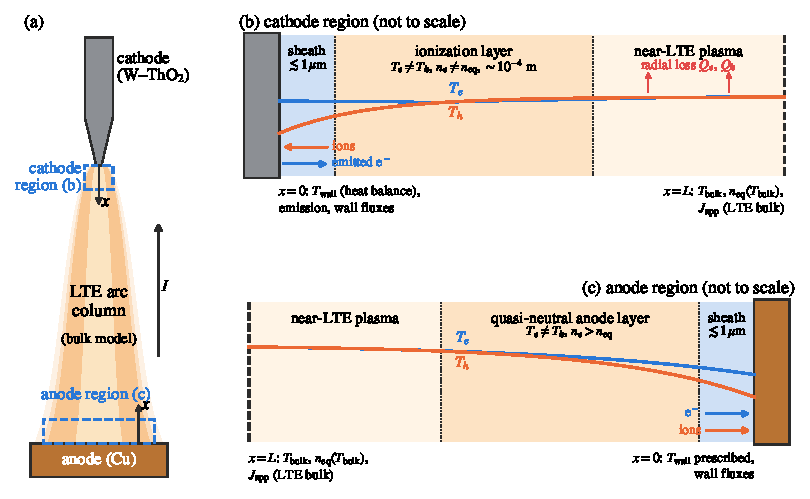
\includegraphics[width=\textwidth]{figures/schematic/arc_schematic.pdf}
\caption{Schematic of the arc discharge and the modeled near-electrode regions.}
\label{fig:schematic}
\end{figure}

\section{Physical model and scale analysis}
\label{sec:model}

\subsection{Governing equations}
\label{sec:model-governing}

In the electrode region, the plasma interacts with the relatively cold, absorbing electrode surfaces. This interaction introduces strong gradients in the plasma properties, causing the plasma to progressively depart from LTE.  We consider plasma to be composed of electrons, singly-charged ions, and neutral atoms for the model. The presence of multiply charged species is neglected as justified in \cite{almeida2000simulation}. To estimate the characteristic length scales associated with these departures, we consider the adjacent LTE plasma at two representative temperatures, \(T=10{,}000~\mathrm{K}\) and \(T=20{,}000~\mathrm{K}\), which are typical of the anode and cathode regions, respectively, in a high-intensity atmospheric-pressure arc discharge \cite{Lowke2006,Hsu1983,LiangTrelles}.

In an ionized gas, the electron mean free path can be approximated as \(\lambda_e = 1/(n_e\overline{Q}_{ee}+n_a\overline{Q}_{ea})\), where \(n_e\) and \(n_a\) are the electron and neutral-atom number densities, respectively, and \(\overline{Q}_{ee}\) and \(\overline{Q}_{ea}\) are the corresponding momentum-transfer collision cross sections for electron--electron and electron--atom collisions. Electron--electron collisions are Coulomb collisions, for which the averaged momentum-transfer cross section is given by \(\overline{Q}_{ee}=e^4\ln\Lambda/[32\pi\varepsilon_0^2(k_BT_e)^2]\) \cite{mitchner1973partially}. Here, \(\ln\Lambda\) is the Coulomb logarithm, given by \(\ln\Lambda=1.24\times10^7 T_e^{3/2}n_e^{-1/2}\), where \(T_e\) is in K and \(n_e\) is in \(\mathrm{m}^{-3}\).

The average electron--neutral momentum-transfer cross section is of the order \(0.2\times10^{-19}~\mathrm{m}^2\) \cite{lxcat} for the electron temperatures considered. Using the corresponding LTE electron and neutral densities, the resulting electron mean free path is of order \(\lambda_e\sim10^{-6}~\mathrm{m}\) in the electrode regions. The characteristic length scale for electron--heavy-particle energy relaxation, \(\lambda_T\), is approximated as\(\frac{\lambda_e}{\sqrt{2M/m_e}}\sim2\times10^{-4}~\mathrm{m}\), where \(M\) is the mass of the heavy species (argon in this case) and \(m_e\) is the electron mass. Thus, \(\lambda_T\sim10^{-4}~\mathrm{m}\).Lowke and Tanaka \cite{Lowke2006} identified a characteristic diffusion length scale for the electron and ion densities of \(\lambda_d\sim10^{-4}~\mathrm{m}\) in the electrode regions.

At the smallest spatial scale, the Debye length calculated from the LTE number densities is of order \(\lambda_{De}\sim10^{-8}~\mathrm{m}\), which characterizes the spatial extent over which charge separation and space-charge effects become important. The ion mean free path provides another relevant scale and can be estimated as \(\lambda_i=1/(n_a\overline{Q}_{ia})\), where \(\overline{Q}_{ia}\) is the momentum-transfer cross section for ion--atom collisions. For argon, we use the approximate fit \(\overline{Q}_{ia}=2[7\times10^{-10}-0.6\times10^{-10}\ln(2k_BT_h)]\) \cite{benilov1998ionization}, where \(k_B\) is the Boltzmann constant and \(T_h\) is the heavy-particle temperature. Since the heavy particle temperature vary from LTE condtions $\sim 1000 \mathrm{K}$ to $\sim 1000 \mathrm{K}$, to electrode temp and since we are interested in region close to the electrode, we use a  temperature of \(T_h\sim1000~\mathrm{K}\), which gives an ion mean free path of order \(\lambda_i\sim10^{-7}~\mathrm{m}\).

The resulting hierarchy of characteristic length scales in the near-electrode region is therefore \(\lambda_{De}\ll\lambda_i\ll\lambda_e\ll\lambda_d\sim\lambda_T\). These estimates indicate that the near-electrode region over which significant departures from LTE develop extends over a characteristic length scale of order \(10^{-4}~\mathrm{m}\). Other modeling results results and analysis shows the same \cite{Almeida2008,DinulescuPfender1980,benilov1995model,hsu1983analysis}. Consistent with this estimate, Lowke and Tanaka \cite{Lowke2006} showed that excluding a near-electrode region of approximately \(10^{-4}~\mathrm{m}\) is sufficient to model the remaining plasma using an LTE approximation. This separation of scales provides the basis for treating the bulk arc with an LTE model while explicitly resolving the nonequilibrium physics in the near-electrode region with a 1D model due to the small size of the near-electrode region.



We therefore model the electrode region as a one-dimensional domain, with the electrode surface at one end and the bulk plasma at the other. Within this region, fluid-dynamic effects associated with bulk plasma motion are neglected, since the near-electrode region is typically contained within the hydrodynamic boundary layer adjacent to the electrode. The neutral species are assumed to be stationary and in thermal equilibrium with the electrode surface and with each other. The ions are assumed to remain in thermal equilibrium with the neutrals because their mean free path is small compared with the characteristic length scale of the temperature variation. Accordingly, the heavy-particle temperature is prescribed using an exponential profile that decreases from the bulk plasma temperature to the electrode temperature,

$$
T_h(x)=T_{\mathrm{bulk}}+\left(T_{\mathrm{wall}}-T_{\mathrm{bulk}}\right)\exp\left(-\frac{x}{L_T}\right),
$$

where \(L_T\) is a characteristic thermal length scale. This exact ion temperature profile makes a little difference on the model because the coliision frequency if ion-neutral has a weak dependence on collision energy. The electron number density and temperature, and the ion number density, are therefore solved self-consistently, while the heavy-particle temperature is prescribed. The neutral number density is not solved independently but is obtained from the ideal-gas law using the prescribed heavy-particle temperature and the constant system pressure. The system is closed by Poisson's equation for the electric potential, which is solved throughout the entire computational domain.

In addition, inertial effects are neglected, and the frictional, pressure-gradient, and electric-field forces are assumed to balance locally for each charged species. This approximation corresponds to a quasi-steady drift-diffusion description in which the species flux adjusts rapidly to changes in the local plasma conditions. It is valid when the momentum-relaxation time is sufficiently short compared with the characteristic timescale of the macroscopic evolution, or equivalently when the associated momentum-relaxation length is small compared with the characteristic spatial scale of the plasma properties. The validity of this approximation is discussed in Section~\textcolor{red}{fill later}. The resulting quasi-steady flux is then used in the species continuity equations to determine the spatial evolution of the charged-particle densities.

The continuity equation for species \(s\) is given by
\begin{equation}
\frac{\partial n_s}{\partial t}+\nabla\cdot\boldsymbol{\Gamma}_s=S_s,
\qquad
\boldsymbol{\Gamma}_s=z_s\mu_s n_s\mathbf{E}-D_s\nabla n_s,
\label{eq:continuity}
\end{equation}
where \(z_s=\pm1\) is the signed charge number, \(\mu_s\) is the mobility, \(D_s\) is the diffusion coefficient, and \(S_s\) is the net ionization--recombination source term. For the simple two-body ionization/recombination scheme considered here, the source terms for electrons and ions are equal in magnitude and opposite in sign. The flux \(\boldsymbol{\Gamma}_s\) is the particle flux of species \(s\); its detailed formulation and the calculation of the corresponding transport properties are described in Appendix~\textcolor{red}{fill later}. The ionization and recombination processes are modeled using the formulation of Hoffert and Lien \cite{hoffert1967quasi}.

The electric field is obtained from Poisson's equation,
\begin{equation}
\nabla\cdot(\varepsilon_0\mathbf{E})=e(n_i-n_e),
\label{eq:poisson}
\end{equation}
which is solved over the entire computational domain, thereby allowing the transition from the quasi-neutral bulk plasma to the space-charge region to be captured without imposing a priori sheath boundaries.

The electron energy is governed by a separate equation of the same convection--conduction--Joule-heating--energy-exchange form commonly used in two-temperature bulk-arc models \cite{HsuPfender1983b,Freton2012},
\begin{equation}
\frac{3}{2}\frac{\partial(n_eT_e)}{\partial t}
+\nabla\cdot\left(\frac{5}{2}T_e\boldsymbol{\Gamma}_e-\kappa_e\nabla T_e\right)
={\mathbf{E}\cdot\mathbf{J}}-\dot{E}_{eh}-\dot{E}_{\rm inel},
\label{eq:eenergy}
\end{equation}
where the terms on the right-hand side represent Joule heating, elastic electron--heavy-particle energy exchange, and inelastic energy losses, respectively. The elastic energy-exchange term is given by \(\dot{E}_{eh}=n_e\delta\nu_{en}\tfrac{3}{2}k_B(T_e-T_{\rm gas})\), where \(\delta=2m_e/M\), while \(\dot{E}_{\rm inel}\) accounts for energy losses associated with inelastic processes, including ionization. Radiation losses are usually small \cite{DinulescuPfender1980,Almeida2008} and thus not included.




Heavy-particle temperature is either taken as a fixed background gas
temperature $T_{\rm gas}(x)$ (the regime in which the present
implementation, Section~\ref{sec:methods}, currently operates) or evolved by
its own energy equation as in \cite{HsuPfender1983b,Almeida2008} when a
fully coupled two-temperature heavy-species treatment is required.


%%%%%%%%%%%%%%%%%%%%%%%%%%%%%%%%%%%%%%%%%%%%%%%%%%%%%%%%%%%%%%%%%%%%%%%%%%%%%%%%%%%
\section{Appendix A. Transport Coefficients}

The electron mobility is obtained from a two-term Boltzmann solution of the BOLSIG+-type, assuming a Maxwellian electron energy distribution, and is tabulated in reduced form as \(\mu_eN(T_e)\) and \(D_eN(T_e)\), rather than being evaluated from a closed-form kinetic-theory expression. This treatment is appropriate in the weakly ionized regime, where electron--neutral collisions dominate and the electron energy distribution is close to Maxwellian. The validity of the Maxwellian assumption is discussed in Section~\textcolor{red}{fill later}. However, in the core region of the arc, particularly near the cathode, electron--ion Coulomb collisions can become significant. To provide a continuous description between these regimes, an electron--ion Coulomb correction is incorporated into the BOLSIG+-based transport coefficients.

The electron--neutral collision frequency is obtained from the BOLSIG+-based mobility as \(\nu_{en}=e/(m_e\mu_{en})\), while the electron--ion collision frequency is calculated using the NRL Plasma Formulary as \(\nu_{ei}=2.91\times10^{-12}n_e[\mathrm{m}^{-3}]\ln\Lambda\,T_e[\mathrm{eV}]^{-3/2}~\mathrm{s}^{-1}\). In the weakly ionized limit, where electron--neutral collisions dominate, the electrical conductivity is \(\sigma_{\rm en}=n_ee^2/(m_e\nu_{en})\), whereas for a fully ionized plasma the electron--ion contribution can be written as \(\sigma_{\rm ei}=1.975\,n_ee^2/(m_e\nu_{ei})\) \cite{mitchner1973partially}. Combining these expressions gives the effective electron mobility
\begin{equation}
\mu_e=\frac{e}{m_e\left(\nu_{en}+\nu_{ei}/1.975\right)}.
\end{equation}
Thus, the BOLSIG+-based electron mobility is corrected by the factor \(\nu_{en}/(\nu_{en}+\nu_{ei}/1.975)\), yielding the effective mobility used in the model. The same correction factor is applied to the electron diffusion coefficient, \(D_e\), to account for the additional momentum loss associated with electron--ion Coulomb collisions. The resulting electrical conductivity is compared with the LTE conductivity in Fig.~\textcolor{red}{fill later}.

The ion--neutral momentum-transfer cross section is obtained from the fitted expression
\(\overline{Q}_{ia}=2[7\times10^{-10}-0.6\times10^{-10}\ln(2k_BT_h)]\) \cite{benilov1998ionization}. The low-field ion mobility is then calculated using the Mason--Schamp equation \cite{mason1958mobility},
\begin{equation}
\mu_i =
\frac{3e}{16N}
\sqrt{\frac{2\pi}{\mu k_B T_{\mathrm{gas}}}}
\frac{1}{\Omega^{(1,1)}(T_{\mathrm{gas}})},
\end{equation}
where \(N\) is the neutral number density, \(\mu\) is the reduced mass of the ion--neutral pair, and \(\Omega^{(1,1)}\) is the corresponding collision integral. This expression gives the ion mobility in the low-field limit, where the ion drift velocity is proportional to the applied electric field.

To account for the field dependence of the ion mobility, a closed-form two-temperature Wannier formulation is employed. The drift velocity is expressed as \(v_d=\mu(T_{\rm eff})E\), where

$$
\mu(T_{\rm eff})=\mu_0\sqrt{\frac{T_{\rm gas}}{T_{\rm eff}}},
\qquad
k_BT_{\rm eff}=k_BT_{\rm gas}+\frac{1}{3}Mv_d^2,
$$

with \(\mu_0\) denoting the low-field mobility and \(M\) the ion mass. Substitution of these relations yields a quadratic equation in \(v_d^2\), which is solved to obtain the field-dependent drift velocity. In the limit \(E\rightarrow0\), the effective temperature approaches the gas temperature, \(T_{\rm eff}\rightarrow T_{\rm gas}\), and the formulation recovers the low-field mobility, \(\mu\rightarrow\mu_0\).




\subsection{Quasi-Maxwellian electrons near the electrode}
\label{sec:model-scaling}

Even where the heavy species are strongly out of equilibrium, the electron
population can remain closely Maxwellian provided electron--electron and
electron--ion collisions are frequent enough to redistribute directed
(drift) energy into the isotropic thermal spread faster than electron--heavy
collisions or the imposed field can distort it. Following Dinulescu and
Pfender's analysis of the anode boundary layer \cite{DinulescuPfender1980},
two conditions must hold. First, electron--electron/ion thermalization must
dominate electron--neutral momentum transfer, weighted by the mass ratio
that makes each electron--neutral collision inefficient at removing energy:
\begin{equation}
\sum_h \frac{m_e}{m_h}\,\frac{\bar\nu_{eh}}{\bar\nu_{ee}} \ll 1 .
\label{eq:maxw1}
\end{equation}
Second, the ordered drift energy imparted by the field must remain small
compared with the electron thermal energy, weighted by the same mass ratio:
\begin{equation}
\left(\frac{U_e}{\bar c_e}\right)^2 \ll \frac{m_e}{m_h} .
\label{eq:maxw2}
\end{equation}
For a representative near-anode condition, $T_e\sim1$~eV, $n_e\sim
5\times10^{22}\,\mathrm{m^{-3}}$, neutral density $N\sim6\times10^{23}\,
\mathrm{m^{-3}}$, electron--atom momentum-transfer cross section
$\bar Q_{ea}=2\times10^{-20}\,\mathrm{m^2}$, and mean thermal speed
$\bar c_e = 7\times10^5\,\mathrm{m/s}$: the electron--ion/electron--electron
frequency from the NRL formulary (with $\ln\Lambda\approx3$) is
$\nu_{ee}\sim\nu_{ei}\sim5\times10^{11}\,\mathrm{s^{-1}}$, while the
electron--neutral frequency is $\nu_{en} = \bar c_e N \bar Q_{ea} \approx
8\times10^{9}\,\mathrm{s^{-1}}$, i.e.\ $\nu_{en}/\nu_{ee}\sim0.016$; with
$m_e/M_{\rm Ar}\approx1.4\times10^{-5}$, condition~(\ref{eq:maxw1}) gives
$\sim2\times10^{-7}\ll1$. For condition~(\ref{eq:maxw2}), the electrical
conductivity of the layer, $\sigma\approx5000$~S/m, corresponds to an
electron mobility $\mu_e = \sigma/(n_e e)\approx0.6\,\mathrm{m^2/(V\,s)}$;
with a representative current density $J\sim10^7\,\mathrm{A/m^2}$, the
electron drift speed is $U_e = J/(en_e) \approx1.3\times10^3\,\mathrm{m/s}$,
so $(U_e/\bar c_e)^2\approx3\times10^{-6}$, again well below
$m_e/M_{\rm Ar}\approx1.4\times10^{-5}$. Both conditions are comfortably
satisfied, so the electron population is treated as quasi-Maxwellian
throughout the near-electrode layer, and a single electron temperature
$T_e$ (rather than a fully kinetic electron energy distribution) is
retained in equation~(\ref{eq:eenergy}) there as well as in the bulk.

\subsection{Length scales and the thickness of the near-electrode layer}
\label{sec:model-lengths}

The same parameters fix a hierarchy of length scales that separates the
space-charge sheath from the broader near-electrode non-equilibrium region
that must be resolved around it. The electron Debye length,
\begin{equation}
\lambda_{De} = \sqrt{\frac{\varepsilon_0 T_e}{n_e e}} \approx 3\times10^{-8}
\ \mathrm{m} ,
\label{eq:debye}
\end{equation}
sets the scale of the space-charge sheath itself. The electron mean free
path against the combined electron--neutral and electron--electron/ion
collision frequency used above,
\begin{equation}
\lambda_e = \frac{\bar c_e}{\nu_{en}+\nu_{ee}} \approx 1\times10^{-6}\
\mathrm{m} ,
\label{eq:mfp}
\end{equation}
is $\sim30$ times $\lambda_{De}$, confirming that the sheath is thin
compared with a mean free path and can support the non-collisional
electron kinetics discussed in Section~\ref{sec:model-collisionality}. The
electron--heavy energy-relaxation length, over which an electron transfers
its excess thermal energy to the heavy gas through the inefficient
mass-ratio-weighted elastic channel in equation~(\ref{eq:eenergy}), is
larger still,
\begin{equation}
\lambda_T = \frac{\lambda_e}{\sqrt{2m_e/M}} \approx 2\times10^{-4}\
\mathrm{m} .
\label{eq:thermal-length}
\end{equation}
Finally, the diffusion length that controls how far the electron/ion density
profile itself can depart from its local equilibrium value under a given
field, used directly by Lowke and Tanaka's mesh-sizing rule
\cite{Lowke2006}, is $\Lambda = (kT_e/e)/E$; with $T_e\approx1$~V and a
field $E = J/\sigma \approx (10^7\,\mathrm{A/m^2})/(5000\,\mathrm{S/m}) =
2000$~V/m consistent with the parameters above,
\begin{equation}
\Lambda \approx 5\times10^{-4}\ \mathrm{m} .
\label{eq:diffusion-length}
\end{equation}
The four scales satisfy $\lambda_{De} \ll \lambda_e \ll \Lambda \sim
\lambda_T$, the same ordering (Debye length $\ll$ mean free path $\ll$
boundary-layer thickness) reported directly in Table~I of
\cite{DinulescuPfender1980} for the anode boundary layer of a comparable
arc, $\lambda_{De}\sim(2$--$3)\times10^{-8}$~m,
$\lambda_e\sim(1$--$2)\times10^{-6}$~m, boundary-layer thickness
$L\sim0.2$--$0.6$~mm. On this basis we take a near-electrode layer of
thickness $\delta \approx 0.2$~mm --- comparable to both $\Lambda$ and
$\lambda_T$, and consistent with the range of $L$ found in
\cite{DinulescuPfender1980} --- as the region over which the unified,
non-equilibrium model of Section~\ref{sec:methods} must be applied; outside
it, the plasma is close enough to collision-dominated equilibrium for the
LTE bulk treatment of Section  to hold. Note that this
$\sim$0.2~mm layer is not itself the space-charge sheath: it is the outer,
thermal/diffusion-dominated non-equilibrium region (corresponding to layers
2--3 of the four-sublayer structure found by \cite{Almeida2008}) inside
which a much thinner space-charge sheath, of order $\lambda_{De}$ to a few
times $\lambda_{De}$, is nested.

\subsection{Is the sheath collisionless?}
\label{sec:model-collisionality}

A collisionless sheath is the standard simplifying assumption used to close
the NLTE-sheath and two-temperature ionization-layer-sheath approaches of
Section~\ref{sec:intro-electrode}, and it is tempting to expect it to hold
automatically at atmospheric pressure, where collision rates are high.
Almeida, Benilov and Naidis show this expectation is wrong: computing the
number of ion collisions actually incurred while crossing the sheath gives
values from order unity to $10^4$, not $\ll1$, even for atmospheric-pressure
argon \cite{Almeida2008}. The reason is that the sheath thickness itself
scales with the \emph{local} Debye length, $\lambda_{De}\propto
n_e^{-1/2}$, which is set by the arc's own high electron density and
shrinks faster, as the arc becomes hotter and more strongly ionized, than
the neutral mean free paths shrink with pressure (the Ramsauer minimum in
the argon electron--neutral cross section keeps $\lambda_e$ from falling as
quickly as $\lambda_{De}$). A collisionless sheath at high pressure is
therefore not evidence of a crude or incomplete model; it is close to the
generic outcome for a dense atmospheric-pressure arc, and the question that
actually needs answering species by species and quantity by quantity is
\emph{how} collisionless, and for what.

We make this quantitative with four Knudsen numbers, each the ratio of the
relevant mean free path to the resolved sheath width $s$: $\mathrm{Kn}_e =
\lambda_e/s$ (do electrons collide crossing the sheath at all);
$\mathrm{Kn}_\varepsilon = \lambda_T/s$ (electron--heavy energy exchange:
does a local electron energy balance exist inside the sheath);
$\mathrm{Kn}_{ee} = \lambda_{ee}/s$ (electron--electron thermalization:
does a well-defined $T_e$, i.e.\ a locally Maxwellian electron energy
distribution, exist inside the sheath at all -- a distinct and much more
restrictive question than $\mathrm{Kn}_\varepsilon$, since $\lambda_{ee}$
and $\lambda_T$ differ by roughly $10^4$); and $\mathrm{Kn}_i =
\lambda_i/s$ for the ion charge-exchange mean free path. For the converged,
resolved-sheath operating point of the \textsc{PlasmeX} test case discussed
in Section~\ref{sec:methods} ($s = 1.65\times10^{-7}$~m $= 5.6\,
\lambda_{De}$, $T_e\approx0.98$~eV at the wall), these evaluate to
$\mathrm{Kn}_e\approx63$, $\mathrm{Kn}_\varepsilon\approx1.2\times10^4$,
$\mathrm{Kn}_{ee}\approx5.3$, and $\mathrm{Kn}_i\approx0.8$--$1.7$: the
sheath is collisionless for electron momentum and electron--heavy energy
exchange by a wide margin, only marginally collisionless for electron
thermalization, and carries of order one ion collision, consistent with the
lower end of the $10^2$--$10^4$ range quoted by \cite{Almeida2008} for a
somewhat different case. Despite $\mathrm{Kn}_{ee}\sim5$ being only
marginal, an electron population entering a purely retarding, elastic
potential barrier is mapped onto itself by Liouville's theorem: reflection
by an energy-conserving barrier preserves a Maxwellian at unchanged $T_e$
while depleting the density by the Boltzmann factor, giving a testable,
parameter-free reference prediction, $T_e(x) = T_{e,\rm edge} = {\rm
const}$ across the sheath, against which the local closure used in
equation~(\ref{eq:eenergy}) can be checked directly (Section~\ref{sec:methods}).
No such collisionless reference state exists for the ions, which do not see
a retarding barrier and for which $\mathrm{Kn}_i = O(1)$ rules out both the
collisionless limit and full collisional equilibrium; ion behaviour in the
sheath is therefore treated as an explicit target for the resolved
drift-diffusion solution rather than assumed a priori in either limit.

\subsection{Boundary conditions}
\label{sec:model-bc}

The system is closed by conditions at the two ends of the domain: the electrode surface, \(x=0\), and the edge of the near-electrode layer, \(x=L\), where the solution is matched to the adjacent LTE bulk plasma. The potential is referenced to zero at the electrode, \(\phi(0)=0\).

\emph{Electrode surface, \(x=0\).} Electrons reaching the surface are absorbed; they are assumed to have a Maxwellian distribution at their local temperature \(T_e\). At the cathode, thermionic emission of electrons, \(\Gamma_{\rm em}\), with a Maxwellian distribution at the wall temperature \(T_{\rm wall}\), is also included. The electron flux into the surface is
\begin{equation}
\boldsymbol{\Gamma}_e\cdot\hat{\mathbf{n}}=\tfrac14n_e\bar c_e-\Gamma_{\rm em},
\qquad
\bar c_e=\sqrt{\frac{8k_BT_e}{\pi m_e}} .
\label{eq:bc-electron}
\end{equation}
The emitted flux is given by the Richardson--Dushman law with Schottky lowering of the work function \(W\) by the field at the surface,
\begin{equation}
\Gamma_{\rm em}=\frac{A_RT_{\rm wall}^2}{e}\exp\!\left(-\frac{W-\Delta W}{k_BT_{\rm wall}}\right),
\qquad
\Delta W=\sqrt{\frac{e^3E_w}{4\pi\varepsilon_0}},
\qquad
E_w=\max(\mathbf{E}\cdot\hat{\mathbf{n}},0),
\label{eq:bc-emission}
\end{equation}
where \(A_R\) is the Richardson constant and \(W\) the work function. Each absorbed electron removes a mean energy \(2k_BT_e\) from the plasma, and each emitted electron brings in \(2k_BT_{\rm wall}\), so the boundary condition for the electron energy equation~(\ref{eq:eenergy}) is
\begin{equation}
\mathbf{h}_e\cdot\hat{\mathbf{n}}=2k_BT_e\,\tfrac14n_e\bar c_e-2k_BT_{\rm wall}\,\Gamma_{\rm em} .
\label{eq:bc-electron-energy}
\end{equation}

Ions reaching the surface are assumed to recombine there and to return to the plasma as atoms. The ion flux into the surface is taken as the sum of a thermal-effusion flux and a directed flux. Let \(\boldsymbol{\Gamma}_i^{d}\) denote the ion flux~(\ref{eq:flux-i}) without its density-diffusion term, \(\boldsymbol{\Gamma}_i^{d}=\boldsymbol{\Gamma}_i+[k_BT_h/(M\bar\nu^M_i)]\nabla n_i\). Ions are absorbed at their thermal-effusion flux plus this directed flux where it points into the wall,
\begin{equation}
\boldsymbol{\Gamma}_i\cdot\hat{\mathbf{n}}=
\tfrac14n_i\bar c_i+\max\!\left(\boldsymbol{\Gamma}_i^{d}\cdot\hat{\mathbf{n}},0\right),
\qquad
\bar c_i=\sqrt{\frac{8k_BT_{\rm wall}}{\pi M}} .
\label{eq:bc-ion}
\end{equation}
Where the sheath field drives the ions into the electrode, the directed term dominates. Elsewhere, the thermal-effusion flux ensures that ions reaching the wall are absorbed even where transport alone does not carry them into it.

The wall is impermeable to the heavy gas, \(\mathbf{u}\cdot\hat{\mathbf{n}}=0\); this is the boundary condition for the heavy-gas momentum equation~(\ref{eq:heavy-momentum}). Equation~(\ref{eq:flux-n}) then gives
\begin{equation}
\boldsymbol{\Gamma}_n\cdot\hat{\mathbf{n}}=-\boldsymbol{\Gamma}_i\cdot\hat{\mathbf{n}} :
\label{eq:bc-neutral}
\end{equation}
every ion neutralized at the surface re-enters the plasma as an atom. Secondary electron emission by ion impact is not included.

The heavy-particle temperature at the surface equals the electrode temperature, \(T_h(0)=T_{\rm wall}\). At the cathode, \(T_{\rm wall}\) is obtained by balancing the heat flux \(q_w\) delivered by the plasma against steady conduction through the cathode body,
\begin{equation}
q_w=\frac{k_w}{L_w}\left(T_{\rm wall}-T_0\right),
\label{eq:bc-heat-balance}
\end{equation}
where \(k_w\) is the thermal conductivity of the cathode, \(L_w\) its length, and \(T_0\) the temperature of its base. This crude heat balance is intended only to capture the trend of the cathode temperature with the current. The anode is usually water-cooled, so its surface temperature is assumed to be constant.

The heat flux into the surface is
\begin{equation}
q_w=\left(2k_BT_e+W\right)\tfrac14n_e\bar c_e
-\left(2k_BT_{\rm wall}+W\right)\Gamma_{\rm em}
+\left(\varepsilon_{\rm ion}-W\right)\boldsymbol{\Gamma}_i\cdot\hat{\mathbf{n}}
-\kappa_h\nabla T_h\cdot\hat{\mathbf{n}} .
\label{eq:bc-qwall}
\end{equation}
The first term is the energy delivered by the absorbed electrons: their kinetic energy plus the work function released on entering the metal.
 The second is emission cooling: each emitted electron removes the work function and its kinetic energy. The third is the energy released when an ion recombines at the surface, \(\varepsilon_{\rm ion}\), less the work function spent to extract the neutralizing electron. The last is heat conduction from the heavy gas. At the anode, \(\Gamma_{\rm em}=0\) and the emission term vanishes.

\emph{Bulk-plasma edge, \(x=L\).} The electron and ion densities and both temperatures are set to Dirichlet values from the adjacent LTE bulk plasma: \(n_e=n_e^{\rm bulk}\), \(n_i=n_i^{\rm bulk}\), and \(T_e=T_h=T_{\rm bulk}\); the last of these is the boundary condition for both energy equations. The neutral density follows from Dalton's law at the background pressure \(p_0\),
\begin{equation}
n_n=\frac{p_0-n_ek_BT_e}{k_BT_h}-n_i .
\label{eq:bc-neutral-density}
\end{equation}
This edge is open to the heavy gas: the heavy-gas momentum equation~(\ref{eq:heavy-momentum}) sees the bulk state, and hence the pressure \(p_0\), outside the boundary, and the heavy-gas velocity is given a zero normal gradient. The arc current is imposed through the electric field in Poisson's equation~(\ref{eq:poisson}): the total current density at the boundary, conduction plus displacement, is held equal to the applied current density \(J_{\rm app}\),
\begin{equation}
e\left(\boldsymbol{\Gamma}_i-\boldsymbol{\Gamma}_e\right)+\varepsilon_0\frac{\partial E}{\partial t}=J_{\rm app},
\label{eq:bc-current}
\end{equation}
which is integrated in time as an evolution equation for the boundary field. 
\subsection{Numerical implementation}
\label{sec:numerics}

The model is solved with a finite-volume code built on the block-structured adaptive mesh refinement framework AMReX \cite{amrex2019}. The domain \(0\le x\le L\) is divided into cells, and the cell averages of \(n_e\), \(n_i\), \(n_n\), \(\mathcal{E}\), \(T_h\), \(\rho u\) and \(\phi\) are the discrete unknowns. Every conservation law is written in flux form, with the fluxes evaluated on the cell faces. The species fluxes~(\ref{eq:flux-e}) and (\ref{eq:flux-i}) are split into a density-diffusion part, \(-D\,\partial n/\partial x\), and a non-diffusive part, \(nv\), where the velocity \(v\) collects the drift in the field, the temperature-gradient and thermal-force terms, the mixture force and the collisional drag. In the sheath, the drift and diffusion fluxes of the electrons nearly cancel, and their sum is two to three orders of magnitude smaller than either. A small relative error in either part would therefore be a large error in the net flux. The face flux is accordingly the exponentially fitted (Scharfetter--Gummel) flux \cite{scharfetter1969},
\begin{equation}
\Gamma_{f}=\frac{D_f}{\Delta x}\Big[B(-\psi)\,n_{\rm L}-B(\psi)\,n_{\rm R}\Big],
\qquad
\psi=\frac{v_f\,\Delta x}{D_f},
\qquad
B(\psi)=\frac{\psi}{e^{\psi}-1},
\label{eq:sg}
\end{equation}
where L and R denote the cells on either side of the face and \(\psi\) is the cell Péclet number. Equation~(\ref{eq:sg}) is exact for the exponential profile of a Boltzmann balance; it reduces to central differencing as \(\psi\to0\) and to upwinding as \(|\psi|\to\infty\). The enthalpy part of the electron energy flux~(\ref{eq:heatflux-e}) is computed from this discrete electron flux, \(\tfrac52k_BT_e\,\Gamma_{e,f}\), so that each electron crossing a face carries exactly its own enthalpy. Heat conduction in both energy equations and Poisson's equation~(\ref{eq:poisson}) are discretized with central differences, and the face field \(E_f=-(\phi_{\rm R}-\phi_{\rm L})/\Delta x\) is used in every face flux and in the Joule heating. The heavy-gas momentum equation~(\ref{eq:heavy-momentum}) is discretized with a Roe-type flux \cite{roe1981}. At the electrode, the wall fluxes~(\ref{eq:bc-electron})--(\ref{eq:bc-neutral}) are imposed as the face fluxes, evaluated with the densities and temperatures of the cell adjacent to the wall; at \(x=L\), the Dirichlet values of Section~\ref{sec:model-bc} are imposed on the boundary face.

All cases in this study use a uniform base mesh of 512 cells with four levels of refinement towards the electrode, each with a refinement ratio of 4. The refined regions are nested layers adjacent to the electrode, \(1.0\times10^{-4}\), \(2.0\times10^{-6}\), \(7.3\times10^{-7}\) and \(2.7\times10^{-7}\)~m deep, with cell sizes of 244, 61, 15.3 and 3.8~nm, so that the mesh has 944 cells in total. These sizes are chosen to resolve the length scales estimated in Section~\ref{sec:scales involved}, down to a fraction of the Debye length, at both the cathode and the anode. The levels are coupled conservatively. The equations are advanced in time, from a uniform initial state at the bulk-plasma conditions or from a neighboring steady state, until a steady state is reached. All equations, including Poisson's equation and the galvanostatic condition~(\ref{eq:bc-current}), are solved together at each time step. A run is considered steady when, for each of \(\phi\), \(n_e\), \(n_i\), \(\mathcal{E}\) and \(T_h\), the relative change over a time step, \(\|\mathbf{U}^{n+1}-\mathbf{U}^{n}\|_2/\|\mathbf{U}^{n+1}\|_2\), extrapolated to \(1\ \mu\)s of simulated time, stays below \(10^{-5}\) on several consecutive checks. The steady states are checked a posteriori by the residual of the electron energy equation and by the uniformity of the total current density (Section~\ref{sec:results}).

\section{Validation}
\label{sec:validation}

The model is validated against two published unified models of the near-electrode layers of atmospheric-pressure argon arcs: the near-cathode layer computed by Almeida et al.\ \cite{Almeida2008} and the near-anode layer computed by Semenov et al.\ \cite{semenov2016numerical}. Both works solve the multi-fluid equations for electrons, ions and atoms, with separate electron and heavy-particle temperatures, coupled to Poisson's equation. The two models differ, however, in geometry. Semenov et al.\ use a planar one-dimensional model, as the present one does, so the current density is the same at every \(x\). Almeida et al.\ instead solve their equations in spherical symmetry about a hemispherical cathode of radius \(r_c=1\)~mm, so their current density decreases with distance as \(j_c\,r_c^2/(r_c+x)^2\), whereas the present model keeps \(j=j_c\) throughout. At the outer boundary of their domains, which is 1~cm from the electrode, both assume that the plasma is uniform and in LTE, with Joule heating balanced by radiation alone. Their solutions show, however, that the plasma is already close to LTE much nearer the electrode: at \(x=5\times10^{-4}\)~m, \(T_e\) and \(T_h\) differ by less than 0.3\,\% in both published solutions, and the charged-particle density is within 2\,\% of the Saha density, although the plasma there is not yet uniform. We therefore restrict the present domain to this length and take the boundary condition at \(x=L\) from the published solutions.

The conditions of the published calculations were reproduced as closely as possible. The electrode surface temperature was prescribed at the value used by Almeida et al.\ and Semenov et al., respectively, rather than obtained from the heat balance~(\ref{eq:bc-heat-balance}), and the radial loss~(\ref{eq:radial-loss}) was switched off, \(\Lambda=0\), since neither model includes it. The domain was discretized as described in Section~\ref{sec:numerics}. Throughout the space-charge sheath, the region where \(|n_i-n_e|/n_i>1\,\%\) (\(x\lesssim1.1\ \mu\)m at the cathode and \(0.7\ \mu\)m at the anode), the cells are smaller than the local electron Debye length, by a factor of at least 1.5 at the cathode and 6 at the anode. The equations were integrated in time at a fixed current density to a steady state. 

\begin{figure}[t]
\centering
\begin{minipage}[t]{0.485\textwidth}
\centering
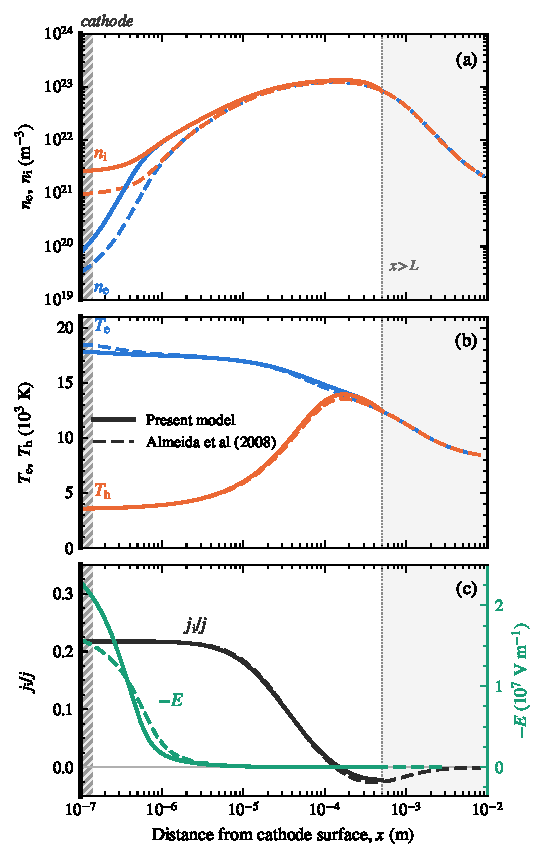
\includegraphics[height=10.5cm]{figures/validation_fig/almeida_J1e7/compareJ1e7_plt00800.pdf}
\caption{Near-cathode layer in argon at atmospheric pressure, cathode surface temperature \(T_{\rm w}=3500\)~K and current density \(j_c=10^7\ \mathrm{A\,m^{-2}}\): present model (solid lines) and Almeida et al.\ \cite{Almeida2008} (dashed lines, figures~5(b) and 6). (a) Electron and ion number densities. (b) Electron and heavy-particle temperatures. (c) Ion fraction of the current density, \(j_i/j\) (left axis), and field strength \(-E\) (right axis). The hatched strip at the left marks the cathode surface. The shaded region, \(x>L\), lies outside the computational domain.}
\label{fig:val-cathode}
\end{minipage}\hfill
\begin{minipage}[t]{0.485\textwidth}
\centering
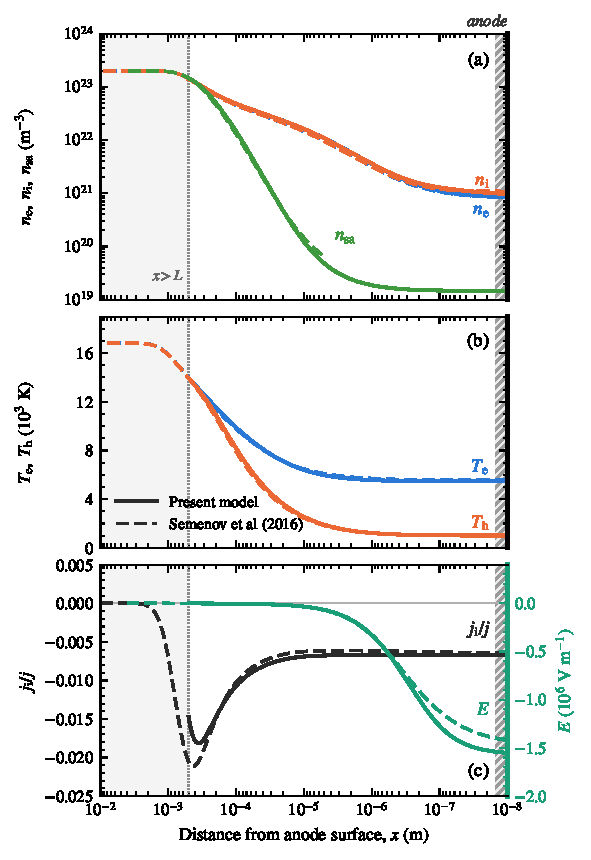
\includegraphics[height=10.5cm]{figures/validation_fig/semenov_J1.5e7/compareJ1.5e7_plt00340.pdf}
\caption{Near-anode layer in argon at atmospheric pressure, anode surface temperature \(T_{\rm s}=1000\)~K and current density \(j=1.5\times10^7\ \mathrm{A\,m^{-2}}\): present model (solid lines) and Semenov et al.\ \cite{semenov2016numerical} (dashed lines, figures~3(b), 4 and 5). (a) Electron and ion number densities and the Saha density \(n_{\rm sa}\). (b) Electron and heavy-particle temperatures. (c) Ion fraction of the current density, \(j_i/j\) (left axis), and electric field \(E\) (right axis). The distance axis is reversed, so that the anode surface, marked by the hatched strip, is at the right. The shaded region, \(x>L\), lies outside the computational domain.}
\label{fig:val-anode}
\end{minipage}
\end{figure}

\subsection{Near-cathode layer}
\label{sec:val-cathode}
Almeida et al.\ \cite{Almeida2008} computed the near-cathode layer of an atmospheric-pressure argon arc for three current densities, and concluded that only one of these cases is realizable in practice: a tungsten cathode with a work function of \(4.55\)~eV, thermionic emission~(\ref{eq:bc-emission}) included, a surface temperature of \(3500\)~K and a current density of \(10^7\ \mathrm{A\,m^{-2}}\). We therefore model this case; the two solutions are compared in figure~\ref{fig:val-cathode}. The temperature profiles agree closely across the whole layer (figure~\ref{fig:val-cathode}(b)). The electron temperature stays near \(17.5\)--\(18\)~kK through the sheath and the inner part of the ionization layer and decreases towards the bulk plasma, while the heavy-particle temperature rises from the wall value to a maximum of \(13.9\)~kK at \(x\approx2\times10^{-4}\)~m, compared with \(13.6\)~kK in the solution of Almeida et al. From \(x\approx3\times10^{-6}\)~m outwards, both temperatures agree with theirs within \(0.4\)~kK (3\,\%).

The ion fraction of the current, figure~\ref{fig:val-cathode}(c), is reproduced over the whole layer. At the cathode surface the present model gives \(j_i/j=0.218\), compared with \(0.216\) reported by Almeida et al.; \(j_i/j\) stays at this value through the sheath, falls to zero at \(x\approx1.5\times10^{-4}\)~m, and becomes slightly negative further out, where the ion flux is directed away from the cathode. Almeida et al.\ also place the sheath edge where the charge separation reaches 1\,\%. The present model gives a sheath voltage of \(9.96\)~V at \(x_{\rm s}=1.1\ \mu\)m, compared with \(10.2\)~V at \(x_{\rm s}=1.5\ \mu\)m in their solution. In the ionization layer, \(10^{-5}\lesssim x\lesssim3\times10^{-4}\)~m, the charged-particle densities of the present model are 7--15\,\% higher than theirs (figure~\ref{fig:val-cathode}(a)). The largest differences are in the space-charge sheath, \(x\lesssim10^{-6}\)~m. At \(x=10^{-7}\)~m, the electron and ion densities of the present model are higher by a factor of about 2.5, and the field strength is \(2.3\times10^7\ \mathrm{V\,m^{-1}}\), compared with \(1.6\times10^7\ \mathrm{V\,m^{-1}}\).



\subsection{Near-anode layer}
\label{sec:val-anode}

The anode case is that of figure~3(b) of Semenov et al.\ \cite{semenov2016numerical}: a non-emitting anode, \(\Gamma_{\rm em}=0\), with surface temperature \(1000\)~K and current density \(1.5\times10^7\ \mathrm{A\,m^{-2}}\). The comparison is shown in figure~\ref{fig:val-anode}. The electron and ion densities agree with those of Semenov et al.\ within 15\,\% across the layer (figure~\ref{fig:val-anode}(a)). Following Semenov et al., the figure also shows the Saha density \(n_{\rm sa}\), the charged-particle density that the local \(T_e\) and \(T_h\) would give in ionization equilibrium with quasi-neutrality at the pressure \(p_0\). Near the anode the actual densities exceed \(n_{\rm sa}\) by nearly two orders of magnitude. The anode region is therefore far from ionization equilibrium: charged particles are supplied by diffusion from the hotter plasma rather than produced locally, and both models capture this departure.

The temperature profiles agree closely (figure~\ref{fig:val-anode}(b)). At the anode surface, the electron temperature is \(5.46\)~kK, compared with \(5.59\)~kK reported by Semenov et al., and the heavy-particle temperatures differ by less than \(0.3\)~kK across the layer. The electric field near the anode, figure~\ref{fig:val-anode}(c), is negative: it is directed towards the anode, so that the anode lies at a lower potential than the adjacent plasma and the electrons are retarded. The field at the surface is \(-1.57\times10^6\ \mathrm{V\,m^{-1}}\), compared with \(-1.42\times10^6\ \mathrm{V\,m^{-1}}\) in the solution of Semenov et al. Ions flow into the anode, so \(j_i/j\) is negative there. At the surface, the present model gives \(j_i/j=-0.0067\), compared with their \(-0.0065\). With the same definition of the sheath edge as at the cathode, the present model gives \(x_{\rm s}=0.70\ \mu\)m and \(\phi_{\rm s}=0.58\)~V, compared with \(0.71\ \mu\)m and \(0.54\)~V obtained from the density and field profiles of Semenov et al.

The main difference is in the minimum of \(j_i/j\), which is \(-0.018\) at \(x=3.5\times10^{-4}\)~m in the present model and \(-0.021\) at \(x=4.3\times10^{-4}\)~m in the solution of Semenov et al. This difference reflects the different models. Imposing their state at \(x=L\) fixes the values of the densities and temperatures there, but not their gradients, which follow from each model's governing equations, and \(j_i/j\) depends on these gradients. 

The present model reproduces the structure of the near-electrode layer for both cathode and anode cases: the temperatures, the current partition between ions and electrons, the sign and magnitude of the near-electrode field, the sheath voltages (within 2.5\,\% at the cathode and 7\,\% at the anode) and the departure from ionization equilibrium. Apart from the charged-particle densities in the cathode sheath and the minimum of \(j_i/j\) near the outer boundary of the anode calculation, the temperatures agree within 3--5\,\% and the charged-particle densities within 15\,\%. The differences most likely arise from the different descriptions of the transport properties (Appendix~\ref{app:transport}) and of the ion boundary condition~(\ref{eq:bc-ion}).

\section{Results}
\label{sec:results}

The model is now applied to an anode and a cathode of a high-intensity arc in argon at atmospheric pressure. The two base cases differ in the bulk-plasma state at \(x=L\), in the current density and in electron emission (table~\ref{tab:base}). Unlike the validation cases of Section~\ref{sec:validation}, the radial loss~(\ref{eq:radial-loss}) is included, with the reactive conductivity in the electron channel. The calibration~(\ref{eq:radial-calibration}) gives a column radius \(R=2.3\)~mm for the anode and \(0.42\)~mm for the cathode. At the anode bulk temperature, \(\kappa_R=0.59\ \mathrm{W\,m^{-1}\,K^{-1}}\) is comparable to \(\kappa_e=0.76\ \mathrm{W\,m^{-1}\,K^{-1}}\), whereas at 21\,000~K the plasma is almost fully ionized and \(\kappa_R=0.03\ \mathrm{W\,m^{-1}\,K^{-1}}\) is negligible. At \(x=L\) all densities and temperatures are Dirichlet values (Section~\ref{sec:model-bc}). The anode surface temperature is prescribed, \(T_{\rm wall}=1000\)~K. The cathode surface temperature is not prescribed: it follows from the heat balance~(\ref{eq:bc-heat-balance}), with \(k_w=100\ \mathrm{W\,m^{-1}\,K^{-1}}\), \(L_w=1\)~cm and \(T_0=1000\)~K. The electrode material has \(W=2.63\)~eV and \(A_R=3\times10^4\ \mathrm{A\,m^{-2}\,K^{-2}}\). The domain, grid and refinement are those of Section~\ref{sec:validation}. Each case was integrated in time at fixed current density until the relative change of every variable over \(1\ \mu\)s fell below \(10^{-3}\). In both steady states, the sum of the terms of the electron energy equation~(\ref{eq:eenergy}), i.e.\ \(\partial\mathcal{E}/\partial t\), is below \(1.2\times10^{-3}\) of its largest term everywhere, and the total current density is uniform to within \(10^{-8}\).
% Run record (not for the paper): PlasmeX runs/base_case_anode/plt47000 (BDF2, steady at
% t = 46.6 us) and runs/base_case_cathode/plt01584 (backward-Euler pseudo-transient to t = 1 ms;
% relative change ~1e-5 per us at the end), 11 Oct 2026. Both with prob.use_radial_loss = 4
% (Q_e = Lambda (k_e + k_R(T_e))(T_e - T_edge), k_R the Mutation++ LTE table), Dirichlet arc face
% (arc_len_E = 0, arc_len_Theta = 1e-9, plasmex.heavy_arc_bc = 0). The 9 Oct runs without the
% radial loss are in each run directory's no_radial_loss/ (their numbers in
% figures/results_fig/report_no_radial_loss.txt); the older mode-1 runs in radial_loss_on/.
% Figures and the table's numbers: figures/results_fig/base_case.py (output in report.txt).

\begin{table}[!htbp]
\caption{Base cases: conditions (top) and computed electrode quantities (bottom). The sheath edge \(x_{\rm s}\) is the distance from the electrode at which \(|n_i-n_e|/n_i\) falls to \(1\,\%\), and \(\phi_{\rm s}\) is the potential there; \(\phi(L)\) is the potential at the bulk-plasma boundary. Both potentials are relative to the electrode. Fluxes are towards the electrode.}
\label{tab:base}
\centering
\small
\begin{tabular}{lcc}
\hline
 & Anode & Cathode \\
\hline
Current density \(|J_{\rm app}|\) (\(\mathrm{A\,m^{-2}}\)) & \(9\times10^{6}\) & \(1.2\times10^{8}\) \\
Bulk temperature \(T_{\rm bulk}\) (K) & 12\,400 & 21\,000 \\
Bulk electron density \(n_e^{\rm bulk}\) (\(\mathrm{m^{-3}}\)) & \(8.2\times10^{22}\) & \(1.7\times10^{23}\) \\
Thermionic emission & off & on \\
\hline
Surface temperature \(T_{\rm wall}\) (K) & 1000 (prescribed) & 3698 \\
\(T_e\) at the surface (K) & 4900 & 19\,500 \\
\(n_e\), \(n_i\) at the surface (\(\mathrm{m^{-3}}\)) & \(5.2\times10^{20}\), \(4.7\times10^{20}\) & \(2.1\times10^{21}\), \(7.6\times10^{21}\) \\
Sheath edge, \(x_{\rm s}\) (m) & \(8.4\times10^{-7}\) & \(5.7\times10^{-7}\) \\
\(\phi_{\rm s}\), \(\phi(L)\) (V) & 0.41, 2.60 & 4.13, 13.68 \\
Field at the surface (\(\mathrm{V\,m^{-1}}\)) & \(-7.2\times10^{5}\) & \(2.2\times10^{7}\) \\
\(j_i/j\) at the surface & \(-0.0037\) & 0.057 \\
Absorbed electron flux \(\tfrac14n_e\bar c_e\) (\(\mathrm{m^{-2}\,s^{-1}}\)) & \(5.6\times10^{25}\) & \(4.6\times10^{26}\) \\
Emitted electron flux \(\Gamma_{\rm em}\) (\(\mathrm{m^{-2}\,s^{-1}}\)) & -- & \(1.17\times10^{27}\) \\
Ion flux \(\boldsymbol{\Gamma}_i\cdot\hat{\mathbf{n}}\) (\(\mathrm{m^{-2}\,s^{-1}}\)) & \(2.1\times10^{23}\) & \(4.3\times10^{25}\) \\
Heat flux \(q_w\) (\(\mathrm{MW\,m^{-2}}\)) & 38.2 & 27.0 \\
\hline
\end{tabular}
\end{table}

\begin{figure}[p]
\centering
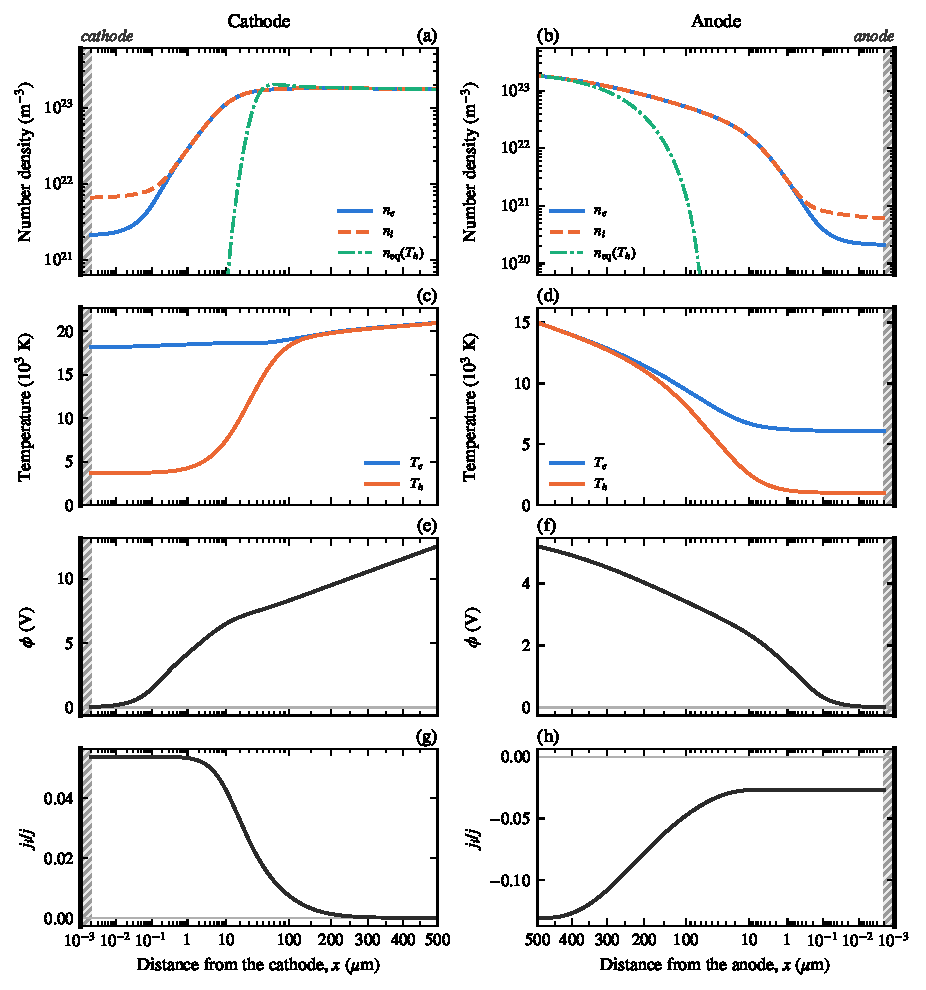
\includegraphics[width=0.92\textwidth]{figures/results_fig/base_profiles.pdf}
\caption{Base cases: cathode (left) and anode (right). \(x\) is the distance from the electrode; the cathode surface is at the left edge of its panels and the anode surface at the right edge of its panels, marked by the hatched strip. The distance axis is scaled as \(\ln x+x/x_c\), with \(x_c=50\ \mu\)m: logarithmic near the electrode and smoothly becoming linear towards the bulk plasma, so that both the sheath and the approach to the bulk are visible. (a), (b) Electron, ion and atom number densities. (c), (d) Electron and heavy-particle temperatures, and the effective ion temperature \(T_{\rm eff}\) of the two-temperature ion mobility (Appendix~\ref{app:transport}), shown where \(n_n>n_i\), the range in which the ion--atom closure applies. (e), (f) Potential relative to the electrode. (g), (h) Ion fraction of the current density, positive for ions flowing into the electrode.}
\label{fig:base-profiles}
\end{figure}

\subsection{Structure of the near-electrode layers}
\label{sec:res-structure}

Figure~\ref{fig:base-profiles} shows the steady profiles of both cases. In both, the plasma departs from LTE over a layer of order \(10^{-4}\)~m, as estimated in Section~\ref{sec:model-governing}, but the structure of this layer is very different at the two electrodes.

\emph{Anode.} The space-charge sheath is practically absent. Charge separation exceeds 1\,\% only within \(0.84\ \mu\)m of the surface, where the potential differs from that of the anode by 0.41~V, and at the surface \(n_e\) exceeds \(n_i\) by 9\,\% (figure~\ref{fig:base-profiles}(b)). The anode lies 2.60~V below the bulk-plasma boundary, and this drop is distributed over the whole quasi-neutral layer (figure~\ref{fig:base-profiles}(f)): 1.14~V within \(10\ \mu\)m, 1.83~V within \(100\ \mu\)m. The field is directed towards the anode and retards the electrons, which reach the surface by diffusion down the steep density gradient: the charged-particle density falls by a factor of 160, from \(8.2\times10^{22}\) to \(5.2\times10^{20}\ \mathrm{m^{-3}}\), across the layer. The electron and heavy-particle temperatures decrease together towards the anode, but \(T_h\) falls faster, to the prescribed surface temperature of 1~kK, so that the two separate progressively: by 2.1~kK at \(x=10^{-4}\)~m, 3.6~kK at \(x=10^{-5}\)~m, and 3.9~kK at the surface, where \(T_e=4.9\)~kK (figure~\ref{fig:base-profiles}(d)). Ions flow into the anode, \(j_i/j<0\), and carry only 0.4\,\% of the current at the surface (figure~\ref{fig:base-profiles}(h)). The field at the anode, \(7.2\times10^5\ \mathrm{V\,m^{-1}}\), is too weak to heat the ions: \(T_{\rm eff}\) exceeds \(T_h\) by about 0.1~kK.

\emph{Cathode.} A space-charge sheath forms, \(0.57\ \mu\)m thick, in which \(n_i\) exceeds \(n_e\) by up to a factor of 3.6 at the surface (figure~\ref{fig:base-profiles}(a)), and across which the potential rises by 4.1~V. The field at the surface is \(2.2\times10^7\ \mathrm{V\,m^{-1}}\). Beyond the sheath, the potential keeps rising through the quasi-neutral ionization layer, to 8.8~V at \(x=10^{-4}\)~m (figure~\ref{fig:base-profiles}(e)). Further out, the plasma approaches the bulk state, and the remaining rise to 13.7~V at \(x=L\) is mostly the ohmic drop of the column, whose field is \(1.1\times10^4\ \mathrm{V\,m^{-1}}\). The electron temperature is nearly uniform, 19.5--21~kK, across the whole layer, while the heavy-particle temperature rises from the surface value of 3.7~kK and approaches \(T_e\) only at \(x\approx10^{-4}\)~m (figure~\ref{fig:base-profiles}(c)). Over the same distance the atom density falls by three orders of magnitude, from \(2\times10^{24}\) to \(2.6\times10^{22}\ \mathrm{m^{-3}}\), and the plasma becomes almost fully ionized. The emitted electron flux, \(1.17\times10^{27}\ \mathrm{m^{-2}\,s^{-1}}\), corresponds to a current density of \(1.9\times10^8\ \mathrm{A\,m^{-2}}\), larger than the arc current density. It is partly returned by the plasma electrons that reach the surface against the sheath field, \(4.6\times10^{26}\ \mathrm{m^{-2}\,s^{-1}}\) (table~\ref{tab:base}), and the ions carry 5.7\,\% of the current at the surface (figure~\ref{fig:base-profiles}(g)). In the sheath, the ions are strongly heated by the field: \(T_{\rm eff}\) reaches 48~kK at the surface (figure~\ref{fig:base-profiles}(c)).

\begin{figure}[!htbp]
\centering
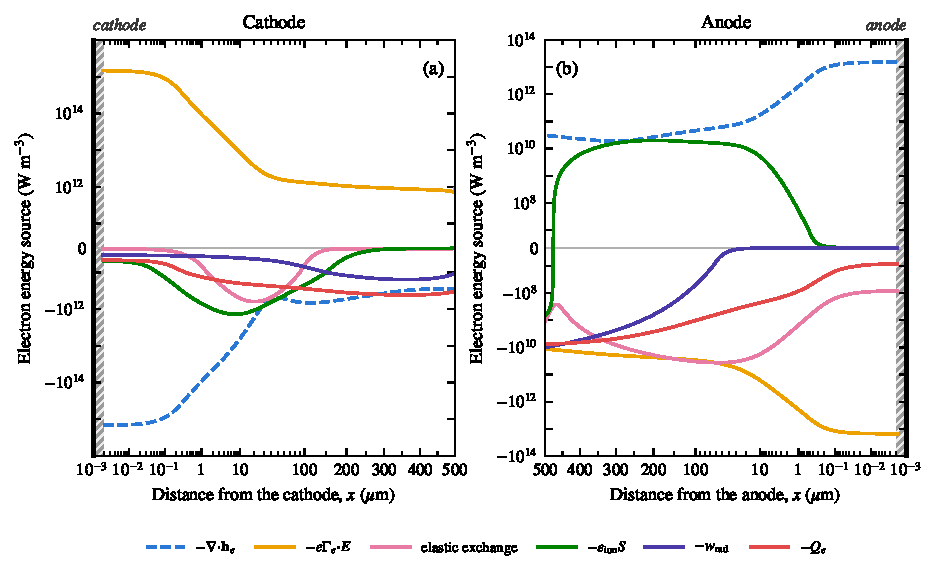
\includegraphics[width=\textwidth]{figures/results_fig/base_een_budget.pdf}
\caption{Steady electron energy balance, equation~(\ref{eq:eenergy}), for (a) the cathode and (b) the anode: every term except \(\partial\mathcal{E}/\partial t\). Dashed: the divergence of the electron energy flux~(\ref{eq:heatflux-e}), \(-\nabla\cdot\mathbf{h}_e\). Solid: the volume terms, i.e.\ Joule heating, elastic exchange with the heavy particles, the ionization sink and the radiative loss. Positive terms heat the electrons. The hatched strip marks the electrode surface: the cathode at the left of panel (a), the anode at the right of panel (b). The distance axis is scaled as \(\ln x+x/x_c\), with \(x_c=50\ \mu\)m: logarithmic near the electrode and smoothly becoming linear towards the bulk plasma, so that both the sheath and the approach to the bulk are visible. The vertical axis is logarithmic in \(|\cdot|\) above \(10^{11}\) (a) and \(10^{6}\ \mathrm{W\,m^{-3}}\) (b), and linear below.}
\label{fig:base-budget}
\end{figure}

\subsection{Electron energy balance}
\label{sec:res-energy}

Figure~\ref{fig:base-budget} compares the terms of the electron energy equation~(\ref{eq:eenergy}) across the layer. The ordering of the terms is again opposite at the two electrodes.

\emph{Anode.} The Joule term \(-e\boldsymbol{\Gamma}_e\cdot\mathbf{E}\) is negative throughout the layer (figure~\ref{fig:base-budget}(b)): the electrons flow towards the anode against the retarding field and lose energy to it, \(23.5\ \mathrm{MW\,m^{-2}}\) over the domain. This loss, and the smaller elastic (\(4.5\ \mathrm{MW\,m^{-2}}\)) and radial (\(2.6\ \mathrm{MW\,m^{-2}}\)) losses, are supplied by the electron energy flux from the column. At \(x=L\), \(36.4\ \mathrm{MW\,m^{-2}}\) flow towards the anode, two thirds of it as the enthalpy flux \(\tfrac52k_BT_e\boldsymbol{\Gamma}_e\), and only \(7.6\ \mathrm{MW\,m^{-2}}\) reach the surface. The convergence of the enthalpy flux, as \(T_e\) falls towards the anode, supplies \(15.0\ \mathrm{MW\,m^{-2}}\), conduction \(4.2\ \mathrm{MW\,m^{-2}}\) and the thermal-diffusion heat flux \(9.6\ \mathrm{MW\,m^{-2}}\). Close to the anode, \(x<10\ \mu\)m, conduction and thermal diffusion provide almost all of the supply, and within \(0.1\ \mu\)m of the surface the thermal-diffusion term alone balances the Joule loss. The volume exchange terms are smaller than the flux terms by two to three orders of magnitude near the anode, and become comparable to them only at \(x\gtrsim10^{-4}\)~m, where the elastic loss to the heavy particles keeps \(T_h\) close to \(T_e\). The ionization term is positive over most of the layer: near the anode the plasma recombines, \(S<0\), because the charged particles are supplied by diffusion at densities well above the local ionization equilibrium (Section~\ref{sec:val-anode}), and the recombination energy heats the electrons.

\emph{Cathode.} Joule heating is the dominant electron energy source everywhere in the layer (figure~\ref{fig:base-budget}(a)). It reaches \(2.5\times10^{15}\ \mathrm{W\,m^{-3}}\) at the surface, where the emitted electrons are accelerated by the sheath field. \(467\ \mathrm{MW\,m^{-2}}\) are deposited in the sheath, and \(1590\ \mathrm{MW\,m^{-2}}\) over the whole domain. In the sheath, the Joule heating is balanced by the divergence of the conduction and thermal-diffusion fluxes (\(334\) and \(113\ \mathrm{MW\,m^{-2}}\)). The electron temperature is slightly lower at the surface than at the sheath edge, 19.5 against 19.7~kK, so these fluxes carry heat towards the cathode. The enthalpy flux of the electron current, directed away from the cathode, is large, 480--540~\(\mathrm{MW\,m^{-2}}\), but nearly uniform, and its divergence is an order of magnitude smaller than that of conduction. Conduction changes sign at \(x\approx1.4\times10^{-5}\)~m and deposits energy in the ionization layer, out to \(x\approx10^{-4}\)~m, where ionization (\(98\ \mathrm{MW\,m^{-2}}\) within \(100\ \mu\)m) and the elastic heating of the heavy particles take it up. Over the whole domain, the Joule heat is distributed as follows: \(690\ \mathrm{MW\,m^{-2}}\) leave at \(x=L\) as electron energy flux into the column (\(543\ \mathrm{MW\,m^{-2}}\) of enthalpy and \(153\ \mathrm{MW\,m^{-2}}\) of thermal-diffusion heat flux); \(574\ \mathrm{MW\,m^{-2}}\) are radial loss, most of it in the column part of the domain, \(x>10^{-4}\)~m; \(130\ \mathrm{MW\,m^{-2}}\) reach the cathode with the absorbed plasma electrons, net of the energy of the emitted electrons; ionization takes \(108\ \mathrm{MW\,m^{-2}}\); and radiation and elastic exchange take \(46\) and \(44\ \mathrm{MW\,m^{-2}}\).

\begin{figure}[!htbp]
\centering
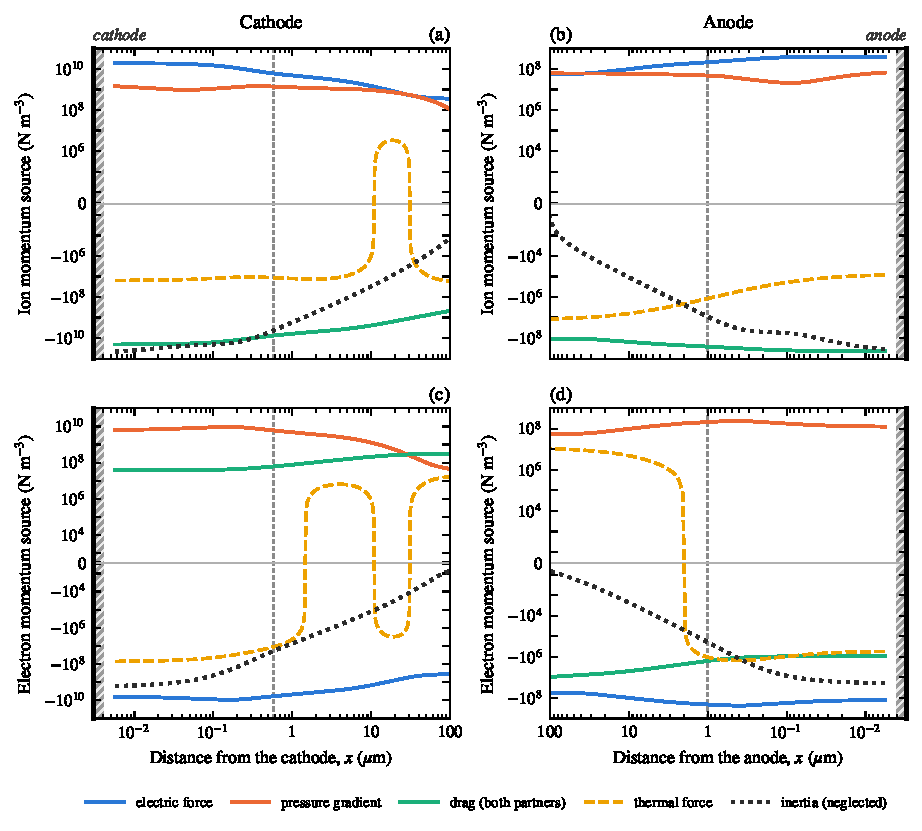
\includegraphics[width=\textwidth]{figures/results_fig/base_momentum.pdf}
\caption{Terms of the steady momentum balances of the ions, equation~(\ref{eq:mom-i}), (a) and (b), and of the electrons, equation~(\ref{eq:mom-e}), (c) and (d), at the cathode (left) and the anode (right), within \(100\ \mu\)m of the electrode. Positive terms push the species towards the electrode. Drag: the friction with both collision partners combined; thermal force: the term in \(C_e\) of equation~(\ref{eq:mom-e}) and its reaction \(C_i\) on the ions. Dotted: the inertia \(-m_sn_s(\mathbf{u}_s\cdot\nabla)\mathbf{u}_s\), which the model neglects, evaluated with \(\mathbf{u}_s=\boldsymbol{\Gamma}_s/n_s\) from the computed fluxes. The vertical dashed line marks the sheath edge \(x_{\rm s}\) (table~\ref{tab:base}). The vertical axis is logarithmic in \(|\cdot|\) and linear within six decades of the largest term.}
\label{fig:base-momentum}
\end{figure}

\begin{figure}[!htbp]
\centering
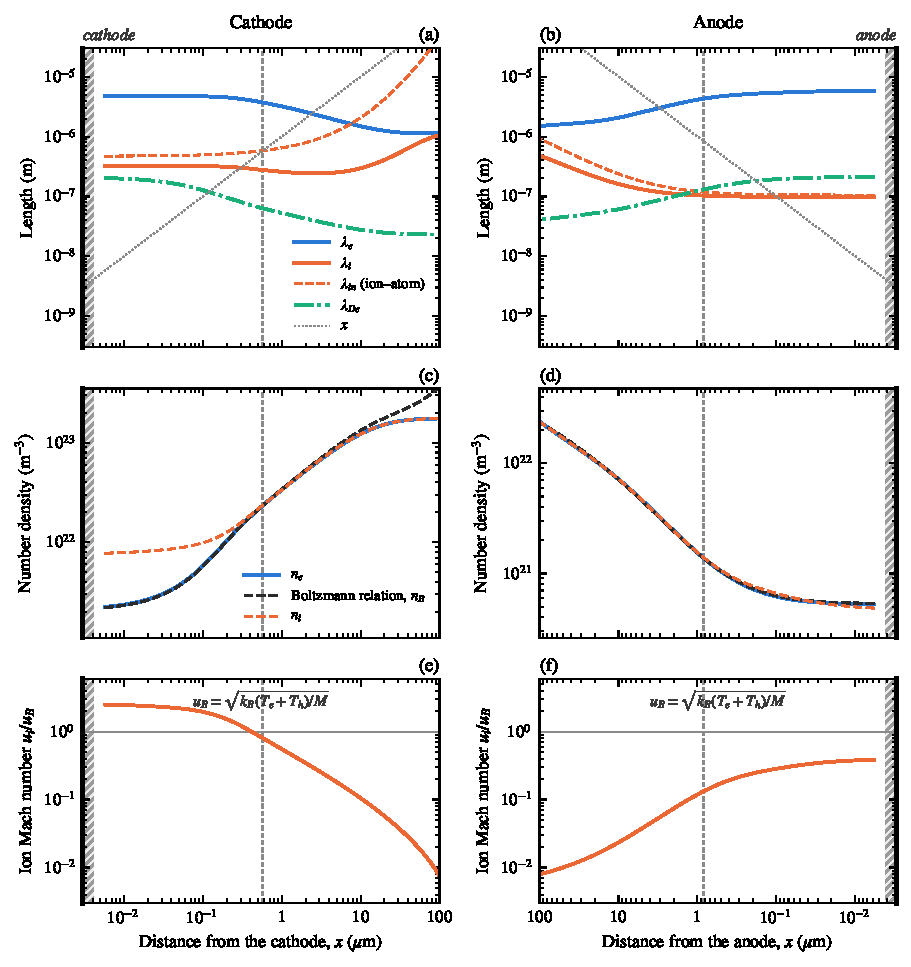
\includegraphics[width=0.92\textwidth]{figures/results_fig/base_sheath.pdf}
\caption{The sheaths of the base cases: cathode (left) and anode (right). (a), (b) Electron and ion mean free paths, the ion--atom part of the latter, and the electron Debye length, from the local state; dotted: the distance \(x\) from the electrode. (c), (d) Electron density and the Boltzmann relation \(n_B=n_e(x_{\rm s})\exp[(e/k_B)\int_{\phi_{\rm s}}^{\phi}d\phi'/T_e]\) started at the sheath edge, with the ion density for reference. (e), (f) Ion velocity towards the electrode, \(u_i=\Gamma_i/n_i\), relative to the Bohm velocity \(u_B=\sqrt{k_B(T_e+T_h)/M}\). The vertical dashed line marks the sheath edge \(x_{\rm s}\).}
\label{fig:base-sheath}
\end{figure}

\subsection{Momentum balance and collisionality of the sheaths}
\label{sec:res-momentum}
% Figures and numbers: figures/results_fig/base_sheath.py (output in base_sheath_report.txt), same plotfiles.

The fluxes~(\ref{eq:flux-e}) and (\ref{eq:flux-i}) follow from the force balances~(\ref{eq:mom-e}) and (\ref{eq:mom-i}), in which the inertia of each species relative to the heavy gas is neglected. Figure~\ref{fig:base-momentum} shows the terms of these balances in the two steady states near the electrode: the electric force, the pressure gradient, the two collisional drags combined, and the thermal force. In the steady states the heavy gas is at rest (\(|\mathbf{u}|\le4\times10^{-4}\ \mathrm{m\,s^{-1}}\) at the cathode and \(0.16\ \mathrm{m\,s^{-1}}\) at the anode), so the share \(Y_s\mathbf{F}\) of the net force is negligible (below \(2\times10^{-4}\) of the largest term). For comparison, the figure also shows the inertia \(m_sn_s(\mathbf{u}_s\cdot\nabla)\mathbf{u}_s\) that the model neglects, evaluated a posteriori from the computed fluxes. The retained terms sum to zero to within \(3\times10^{-3}\) of the largest one.

\emph{Ions.} In both sheaths, the electric force on the ions is balanced by the drag (figure~\ref{fig:base-momentum}(a), (b)). At the cathode the pressure gradient adds at most 22\,\% to the electric force in the sheath, and 7\,\% at the surface. At the anode the field is weaker, and the pressure gradient, which also drives the ions towards the surface, is 68\,\% of the electric force there. The thermal force on the ions is negligible, below 1\,\% of the drag in either sheath. The neglected inertia is not small inside the cathode sheath. It exceeds the drag within \(0.36\ \mu\)m of the surface, by a factor of 2.4 at the surface, and stays above 10\,\% of the drag out to \(2.3\ \mu\)m; beyond \(14\ \mu\)m it is below 1\,\%. At the anode the inertia is at most 35\,\% of the drag, at the surface, and below 10\,\% beyond \(0.09\ \mu\)m.

\emph{Electrons.} In both sheaths the field retards the electrons, and the electric force on them is balanced by their pressure gradient (figure~\ref{fig:base-momentum}(c), (d)). In the sheath the two cancel to within 0.9\,\% (cathode) and 4.7\,\% (anode) of the electric force. The drag (0.6 and 2.6\,\% of the electric force at the surface) and the thermal force (1.2 and 0.9\,\%) are small there. The drag becomes important only in the quasi-neutral layer, where it carries the current: at \(10\ \mu\)m from the surface it is 16\,\% (cathode) and 20\,\% (anode) of the electric force. The inertia of the electrons exceeds their drag within \(0.33\ \mu\)m of the cathode (by up to a factor of 54) and within \(0.59\ \mu\)m of the anode (by up to a factor of 6), but it remains smaller than the electric force: at the surface it is a third of the electric force at the cathode and 16\,\% at the anode, and at the sheath edge 0.3 and 2.3\,\%. At the cathode, this inertia is that of the emitted electrons, accelerated by the sheath field.

\emph{Mean free paths.} Figure~\ref{fig:base-sheath}(a), (b) shows the mean free paths \(\lambda_e\) and \(\lambda_i\) of table~\ref{tab:scales}, evaluated with the local densities and temperatures, the ion--atom part of \(\lambda_i\), \(\lambda_{in}=1/(n_n\overline{Q}_{in})\), and the electron Debye length. The electron mean free path is of order microns, \(3.8\ \mu\)m at the cathode sheath edge and \(4.3\ \mu\)m at the anode one. The sheaths, \(0.57\) and \(0.84\ \mu\)m thick, therefore contain only 0.13 and 0.17 electron mean free paths, and \(\lambda_e\) exceeds the distance from the surface within \(2.3\ \mu\)m of the cathode and \(2.8\ \mu\)m of the anode. The ions are more collisional. At the sheath edge, \(\lambda_i=0.28\ \mu\)m at the cathode and \(0.10\ \mu\)m at the anode, so that the ions cross 1.8 and 8.2 mean free paths in the sheaths (1.05 and 7.4 counting only the collisions with atoms). The anode sheath is thus collision-dominated for the ions, consistent with their small inertia. The cathode sheath is transitional: the ions make one to two collisions across it, and their inertia exceeds the drag over its inner two thirds. There the ions cannot follow the steep rise of the field, and the local relation between field and ion velocity in equation~(\ref{eq:flux-i}) overestimates the ion velocity near the surface. The electrons cross both sheaths practically without collisions. Their balance there is, however, not a balance of collisional transport: the drag is a few per cent of the electric force, and the field and pressure gradient balance each other as in the Boltzmann equilibrium of a Maxwellian population retarded by a potential barrier, which does not require collisions. The electron description therefore remains adequate in the sheaths, except within about \(0.1\ \mu\)m of the cathode, where the inertia of the emitted electrons is no longer small. Beyond 2--3~\(\mu\)m from either electrode, the inertia of both species is below 10\,\% of the drag, and the inertialess, collision-dominated description of section~\ref{sec:model-governing} holds.

\emph{Boltzmann electrons and the Bohm criterion.} Simplified sheath models describe the electrons in the sheath by the Boltzmann relation and impose the Bohm criterion on the ions entering it, \(u_i\ge u_B\), with \(u_B=\sqrt{k_B(T_e+T_i)/M}\). Figure~\ref{fig:base-sheath}(c)--(f) tests both against the computed sheaths. The electron density follows the Boltzmann relation closely. Started at the sheath edge, the relation reproduces \(n_e\) to within 1.5\,\% across the cathode sheath, where \(n_e\) falls by a factor of 10, and to within 2.1\,\% across the anode sheath, where it falls by a factor of 2.6. Outside the anode sheath it still holds to within 2.3\,\% at \(100\ \mu\)m. At the cathode it fails progressively in the ionization layer, where the electron drag carries the current: \(n_e\) is 8\,\% below \(n_B\) at \(10\ \mu\)m and 53\,\% below at \(100\ \mu\)m. The ions, in contrast, do not satisfy the Bohm criterion at the sheath edge (figure~\ref{fig:base-sheath}(e), (f)). At the cathode they enter the sheath at \(u_i=1830\ \mathrm{m\,s^{-1}}\), against \(u_B=2230\ \mathrm{m\,s^{-1}}\), i.e.\ at 0.82\,\(u_B\). They reach \(u_B\) only \(0.40\ \mu\)m from the surface, inside the sheath, where the charge separation is already 2.9\,\%, and arrive at the surface at 2.5\,\(u_B\). At the anode the ions enter the sheath at 0.13\,\(u_B\) and reach the surface at 0.39\,\(u_B\), never attaining \(u_B\). The Bohm flux \(n_iu_B\) at the sheath edge would therefore overestimate the ion flux entering the sheath by 22\,\% at the cathode and by a factor of 7.5 at the anode. The Bohm criterion is derived for a collisionless sheath. In these sheaths the ions collide with the atoms throughout the presheath and the sheath, and, except in the inner part of the cathode sheath, their velocity is set by the balance of the electric force and the drag rather than by the potential drop they have fallen through. This agrees with the conclusion of Semenov et al.\ \cite{semenov2016numerical} for the anode layer.

\begin{figure}[!htbp]
\centering
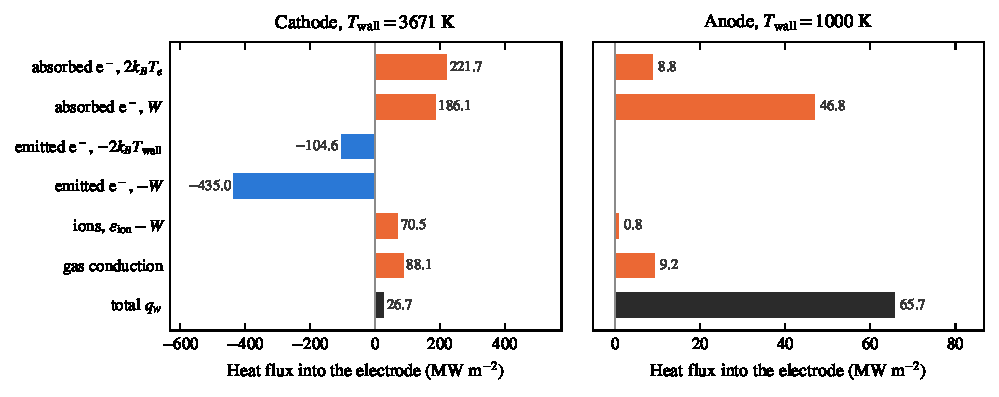
\includegraphics[width=\textwidth]{figures/results_fig/base_qwall.pdf}
\caption{Terms of the heat flux delivered to the electrode, equation~(\ref{eq:bc-qwall}), positive into the electrode, for the cathode (left) and the anode (right). Orange: heating; blue: emission cooling; black: the net heat flux \(q_w\). At the cathode, \(q_w\) equals the conduction \(k_w(T_{\rm wall}-T_0)/L_w\) into the electrode body, equation~(\ref{eq:bc-heat-balance}); the anode surface temperature is prescribed.}
\label{fig:base-qwall}
\end{figure}

\subsection{Heat flux to the electrode}
\label{sec:res-heat}

The terms of the electrode heat flux~(\ref{eq:bc-qwall}) are shown in figure~\ref{fig:base-qwall}. At the anode, \(q_w=38.2\ \mathrm{MW\,m^{-2}}\) and the absorbed electrons deliver 82\,\% of it: 23.8~\(\mathrm{MW\,m^{-2}}\) as the work function released on entering the metal and 7.6~\(\mathrm{MW\,m^{-2}}\) as kinetic energy. Gas conduction contributes \(6.4\ \mathrm{MW\,m^{-2}}\) and ion recombination about 1\,\%. The anode heat flux is thus set by the electron current, through \(W\), and by the electron temperature at the surface; with the surface temperature prescribed, it is the heat that the anode cooling has to remove.

At the cathode, the heat flux is the small difference of large terms. The absorbed plasma electrons (\(443\ \mathrm{MW\,m^{-2}}\)), gas conduction (\(105\ \mathrm{MW\,m^{-2}}\)) and ion recombination (\(90\ \mathrm{MW\,m^{-2}}\)) heat the surface by \(638\ \mathrm{MW\,m^{-2}}\) in total, and emission cools it by \(611\ \mathrm{MW\,m^{-2}}\), so that only \(q_w=27.0\ \mathrm{MW\,m^{-2}}\) is conducted into the cathode body. The surface temperature, 3698~K, is therefore fixed mainly by the condition that emission cooling nearly balances the heating, and only weakly by the conduction into the cathode body. Emission cooling grows with \(T_{\rm wall}\) as \(T_{\rm wall}^2\exp[-(W-\Delta W)/(k_BT_{\rm wall})]\), i.e.\ by about 0.27\,\% per kelvin at this temperature, so a 5\,\% change in the heating would shift \(T_{\rm wall}\) by only about 20~K, and \(q_w\) by less than 1\,\%. Ion recombination, at \(\varepsilon_{\rm ion}-W=13.1\)~eV per ion, provides 14\,\% of the heating, although the ions carry only 5.7\,\% of the current.

\emph{Ion impact energy.} Equation~(\ref{eq:bc-qwall}) charges the ions with their recombination energy only, not with the kinetic energy with which they strike the surface. In the model, the ion energy follows from the local field through the two-temperature closure (Appendix~\ref{app:transport}), which presumes that the ions make many collisions over the distance in which the field changes. The cathode sheath does not satisfy this: the ions cross it with only one to two collisions, and their inertia exceeds the drag over its inner part (Section~\ref{sec:res-momentum}). The local mean ion energy at the cathode surface is therefore not a reliable impact energy, and its distribution would require a kinetic treatment of the sheath. We therefore give only the maximum impact energy at the cathode: that of an ion that enters the sheath with the mean energy at the sheath edge, \(\tfrac32k_BT_{\rm eff}+\tfrac12Mv_d^2=1.5\)~eV (equations~(\ref{eq:wannier}) and (\ref{eq:mu-in})), and crosses it without a collision, gaining \(e\phi_{\rm s}=4.1\)~eV. This maximum is 5.6~eV per ion, and with the ion flux of table~\ref{tab:base} it delivers at most \(38\ \mathrm{MW\,m^{-2}}\), comparable to \(q_w\) itself. Added to the heating, this term would, however, raise \(T_{\rm wall}\) by only about 20~K, most of it being removed by emission cooling, and \(q_w\) by about 1\,\%. At the anode, where the ions carry 0.4\,\% of the current and fall through only 0.41~V in a collision-dominated sheath, their kinetic energy is negligible.


\subsection{Dependence on the bulk temperature and the current density}
\label{sec:res-sweep}
% Run record (not for the paper): PlasmeX runs/base_sweep, 11 Oct 2026 (launch.sh,
% ladder4_J2e8.sh, tighten_and_1p5.sh; what failed is in failed_attempts/). Every run stopped by
% the steady-state trigger; energy residual <= 1.3e-3 of the largest term. Anode: from the base
% state (plasmex.init_plotfile). Cathode: J = 8e7, 9e7 (from the old cathode_sweep 8e7 state), 1e8
% from a steady state, the T series from the uniform initial state, J > 1.2e8 by a 4 % current
% ladder of checkpoint restarts (prob.wall_temp_tau = 1e-6 s from 1.3e8 on; same steady state).
% Above ~1.5e8 no route reached a steady state; the user ended the sweep at 1.5e8. All cathode
% states restarted at steady_tol = 1e-5 (tight/), so the heat balance closes to 9e-4.
% Figures and numbers: figures/results_fig/base_sweep.py (base_sweep.csv).

The base cases were repeated with the bulk temperature varied at fixed current density, \(T_{\rm bulk}=11\,000\)--\(14\,000\)~K for the anode and \(19\,000\)--\(23\,000\)~K for the cathode (figure~\ref{fig:sweep-T}), and with the current density varied at the base bulk temperature, \(|J_{\rm app}|=7\times10^{6}\)--\(2\times10^{7}\ \mathrm{A\,m^{-2}}\) for the anode and \(8\times10^{7}\)--\(1.5\times10^{8}\ \mathrm{A\,m^{-2}}\) for the cathode (figure~\ref{fig:sweep-J}). Everything else is as in the base cases. In particular, \(\Lambda\) is recalibrated for each bulk state through equation~(\ref{eq:radial-calibration}), which gives column radii of 1.0--4.1~mm for the anode cases and 0.33--0.66~mm for the cathode cases.

\begin{figure}[p]
\centering
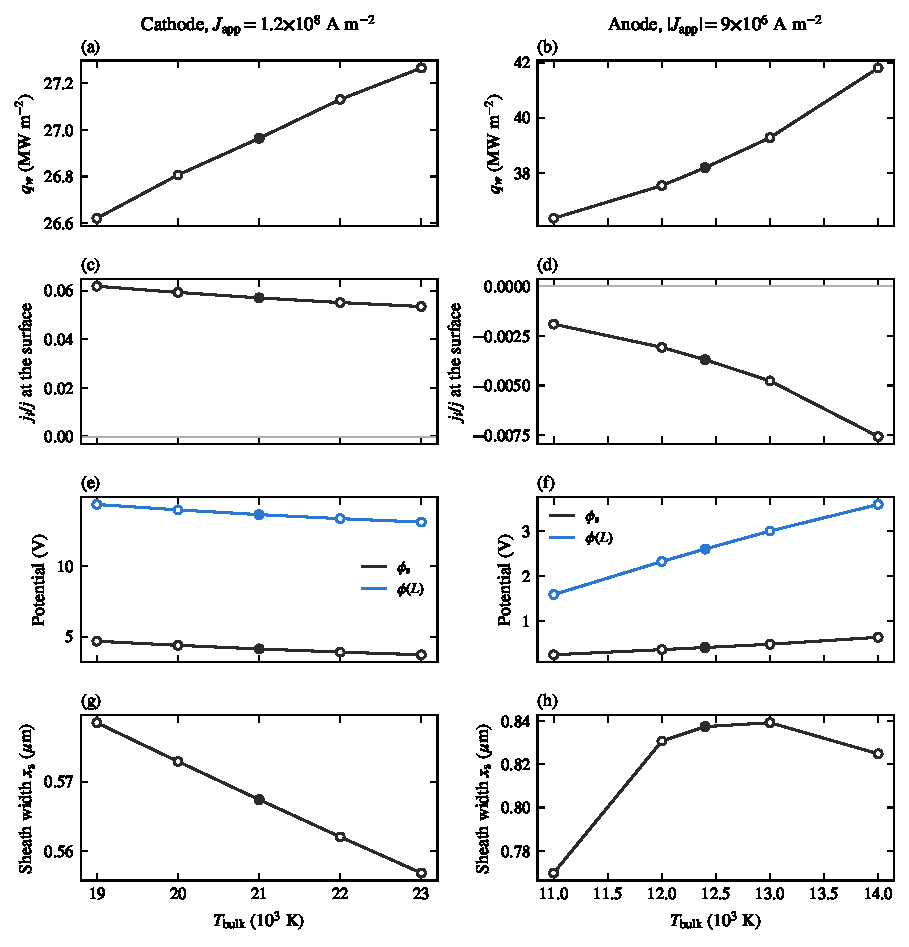
\includegraphics[width=0.92\textwidth]{figures/results_fig/base_sweep_T.pdf}
\caption{Electrode quantities against the bulk temperature \(T_{\rm bulk}\), for the cathode at \(J_{\rm app}=1.2\times10^{8}\ \mathrm{A\,m^{-2}}\) (left) and the anode at \(|J_{\rm app}|=9\times10^{6}\ \mathrm{A\,m^{-2}}\) (right). Filled symbols: the base cases. (a), (b) Heat flux into the electrode \(q_w\), equation~(\ref{eq:bc-qwall}). (c), (d) Ion fraction of the current density at the surface, positive for ions flowing into the cathode; at the anode the ions also flow into the surface, against the current. (e), (f) Potential at the sheath edge \(\phi_{\rm s}\) and at the bulk-plasma boundary \(\phi(L)\), relative to the electrode. (g), (h) Sheath width \(x_{\rm s}\), the distance from the surface at which \(|n_i-n_e|/n_i\) falls to 1\,\%.}
\label{fig:sweep-T}
\end{figure}

\begin{figure}[p]
\centering
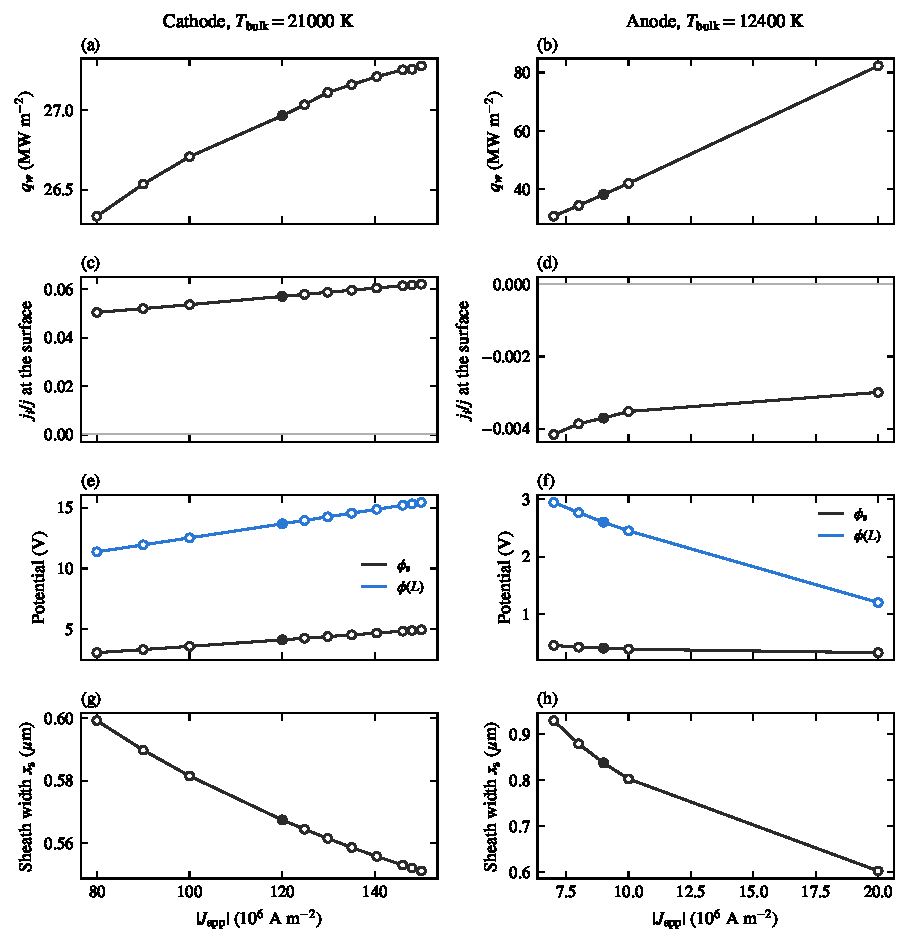
\includegraphics[width=0.92\textwidth]{figures/results_fig/base_sweep_J.pdf}
\caption{As figure~\ref{fig:sweep-T}, against the current density \(|J_{\rm app}|\), for the cathode at \(T_{\rm bulk}=21\,000\)~K (left) and the anode at \(T_{\rm bulk}=12\,400\)~K (right).}
\label{fig:sweep-J}
\end{figure}

\emph{Cathode.} The heat flux to the cathode hardly changes: \(q_w=26.3\)--\(27.3\ \mathrm{MW\,m^{-2}}\) in every case (figures~\ref{fig:sweep-T}(a) and \ref{fig:sweep-J}(a)), while \(T_{\rm wall}\) varies only between 3633 and 3727~K. This follows from the heat balance~(\ref{eq:bc-heat-balance}). With the electrode parameters used here, a change of \(q_w\) by \(1\ \mathrm{MW\,m^{-2}}\) requires a change of \(T_{\rm wall}\) by 100~K, which would change the emission cooling by about 30\,\%. The heating of the surface, by the absorbed electrons, the ions and gas conduction, does depend on the plasma: it increases from 488 to \(735\ \mathrm{MW\,m^{-2}}\) between \(J_{\rm app}=8\times10^{7}\) and \(1.5\times10^{8}\ \mathrm{A\,m^{-2}}\). The surface temperature then rises by only 94~K, and the additional heating is removed by emission cooling. Within these ranges, the heat flux conducted into the cathode is therefore set by the electrode, through \(W\), \(A_R\), \(k_w\), \(L_w\) and \(T_0\), rather than by the plasma. The plasma side adjusts instead. With increasing current density, the sheath drop rises from 3.1 to 5.0~V and the ion fraction of the current at the surface from 5.0 to 6.2\,\% (figure~\ref{fig:sweep-J}). The electron temperature at the surface rises from 16.7 to 21.4~kK, and the voltage across the domain from 11.4 to 15.4~V. The emitted current exceeds the arc current in every case, but by less as the current grows, from 1.77 to 1.44 times the arc current. Above \(1.5\times10^{8}\ \mathrm{A\,m^{-2}}\) no steady state was reached with this cathode heat balance. Increasing the bulk temperature at fixed current acts in the opposite direction on the sheath (figure~\ref{fig:sweep-T}). Between 19\,000 and 23\,000~K, \(\phi_{\rm s}\) decreases from 4.7 to 3.7~V, \(j_i/j\) from 6.2 to 5.3\,\% and \(T_e\) at the surface from 20.3 to 18.9~kK, while the voltage across the domain \(\phi(L)\) falls from 14.4 to 13.1~V. The sheath width changes by less than 10\,\% in either sweep (figures~\ref{fig:sweep-T}(g) and \ref{fig:sweep-J}(g)): it decreases from 0.60 to \(0.55\ \mu\)m as the current density increases, and from 0.58 to \(0.56\ \mu\)m as the bulk temperature increases. The larger sheath drop at higher current is held across a nearly unchanged width by a denser ion space charge: the ion density at the surface rises from \(5.5\times10^{21}\) to \(9.2\times10^{21}\ \mathrm{m^{-3}}\).

\emph{Anode.} The anode heat flux increases almost in proportion to the current density, from 30.7 to \(82.3\ \mathrm{MW\,m^{-2}}\) between \(|J_{\rm app}|=7\times10^{6}\) and \(2\times10^{7}\ \mathrm{A\,m^{-2}}\) (figure~\ref{fig:sweep-J}(b)), i.e.\ 4.4 to 4.1~W per ampere. Of this, the work function released by the absorbed electrons contributes exactly \(W|J_{\rm app}|/e\), i.e.\ 2.63~W per ampere. Their kinetic energy, \(2k_BT_e\) per electron with \(T_e\) at the surface rising from 4.7 to 6.0~kK, contributes another 0.8--1.0~W per ampere. Gas conduction (6.1--\(7.9\ \mathrm{MW\,m^{-2}}\)) and ion recombination (below \(1\ \mathrm{MW\,m^{-2}}\)) contribute the rest. At fixed current, the bulk temperature has a much weaker effect, \(q_w=36.4\) to \(41.8\ \mathrm{MW\,m^{-2}}\) between 11\,000 and 14\,000~K (figure~\ref{fig:sweep-T}(b)). The electron terms are fixed by the current and by \(T_e\) at the surface, which stays between 4.9 and 5.2~kK, and the increase comes mostly from gas conduction, which rises from 4.4 to \(9.1\ \mathrm{MW\,m^{-2}}\). In every anode case, the ions carry less than 1\,\% of the current. The anode lies below the bulk-plasma boundary by \(\phi(L)=1.6\) to 3.6~V as \(T_{\rm bulk}\) increases from 11\,000 to 14\,000~K. With increasing current density this drop decreases, from 2.9~V at \(7\times10^{6}\) to 1.2~V at \(2\times10^{7}\ \mathrm{A\,m^{-2}}\). The potential at the edge of the thin space-charge layer stays between 0.25 and 0.64~V. The width of this layer follows the electron density at the surface. It decreases from 0.93 to \(0.60\ \mu\)m as the current density increases from \(7\times10^{6}\) to \(2\times10^{7}\ \mathrm{A\,m^{-2}}\) (figure~\ref{fig:sweep-J}(h)), while \(n_e\) at the surface rises from \(4.1\times10^{20}\) to \(1.0\times10^{21}\ \mathrm{m^{-3}}\), nearly as \(n_e^{-1/2}\), the scaling of the Debye length. At fixed current, \(n_e\) at the surface changes by at most 3\,\% with the bulk temperature, and the width stays between 0.77 and \(0.84\ \mu\)m (figure~\ref{fig:sweep-T}(h)).

\subsection{Relaxation times}
\label{sec:res-time}

% Run record (not for the paper): PlasmeX runs/base_timescales (README.md there), 11 Oct 2026. Each state of
% the base cases and sweeps re-converged with T_wall and Lambda pinned (steady_tol 1e-7), then |J_app| x 1.02,
% BDF2 at imp_ttol 3e-5. Cathode: plasmex.heavy_inertia 1e-4 (records e1e-4); anode: physical sound (e1), which
% equals heavy_inertia 1e-6 on the base case to 0.2 %. The physical-sound and domain-length records are in
% base_timescales.csv but not in the paper (user, 12 Oct 2026). Figure, csv and the numbers below:
% figures/results_fig/base_timescales.py (output in base_timescales_report.txt).
To estimate how quickly the near-electrode layers follow a change of the arc, each steady state of Sections~\ref{sec:res-structure}--\ref{sec:res-sweep} was perturbed by a step of \(+2\,\%\) in \(|J_{\rm app}|\), and the time-dependent equations were integrated to the new steady state. The surface temperature and the radial-loss coefficient \(\Lambda\) were held at their steady values, since the electrode body responds on a time scale of seconds and \(\Lambda\) represents the column outside the domain. The response of the ion current density \(j_i\) and of the heat flux \(q_w\) at the surface is characterized by the time to steady state \(t_{99}\), after which the quantity stays within 1\,\% of its total change.

In a one-dimensional domain, the step also excites an axial acoustic oscillation of the heavy gas between the electrode and the boundary \(x=L\). In a three-dimensional arc, such a pressure disturbance is relieved radially within \(R/c\approx0.1\ \mu\)s. The axial acoustics are therefore removed by multiplying the inertia of the heavy gas, the left-hand side of equation~(\ref{eq:heavy-momentum}), by \(\epsilon=10^{-4}\). This raises the sound speed to \(c/\sqrt{\epsilon}\) and leaves the steady state, with \(\mathbf{u}=0\), unchanged; \(t_{99}\) varies by less than 3\,\% for \(10^{-6}\le\epsilon\le10^{-3}\). At the anode, the acoustics do not affect the response, and the physical sound speed is retained.

\begin{figure}[!htbp]
\centering
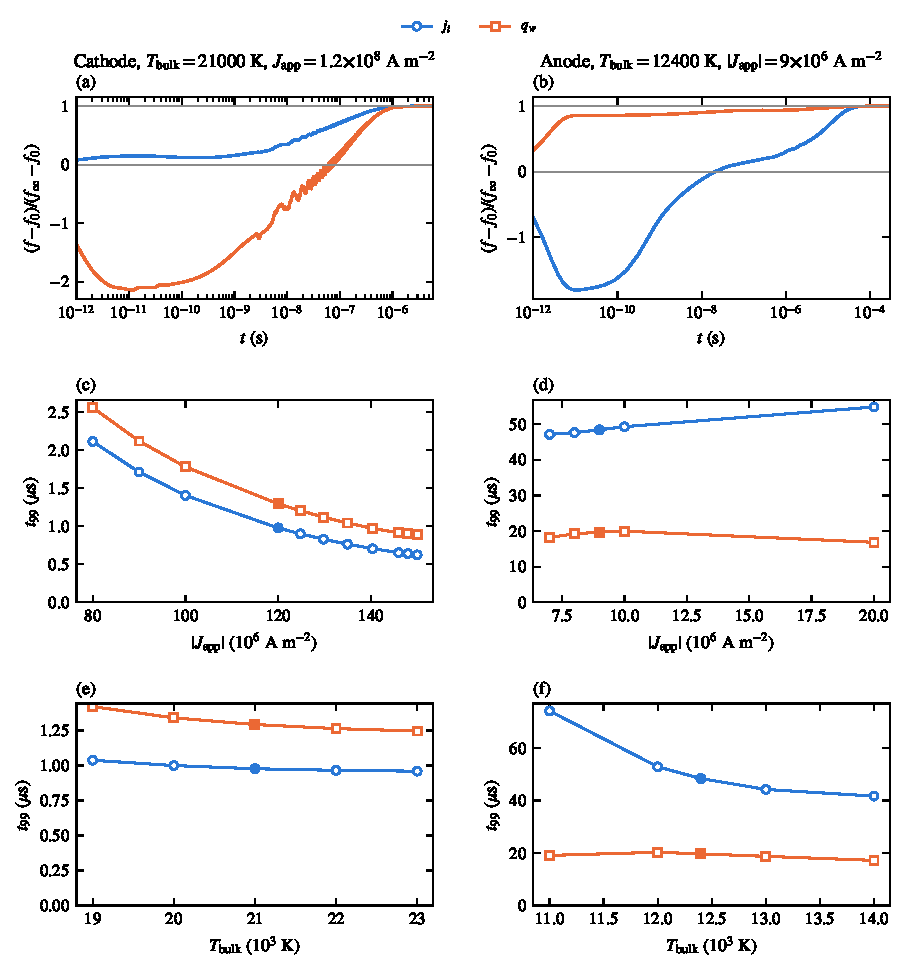
\includegraphics[width=0.92\textwidth]{figures/results_fig/base_timescales.pdf}
\caption{Response of the electrode quantities to a \(+2\,\%\) step of \(|J_{\rm app}|\): cathode (left, axial acoustics removed) and anode (right). Blue: ion current density \(j_i\) at the surface; orange: heat flux \(q_w\) into the surface. (a), (b) Normalized response of the base cases, \(f_0\) and \(f_\infty\) being the initial and the final values. (c), (d) Time to steady state \(t_{99}\) against \(|J_{\rm app}|\) at the base \(T_{\rm bulk}\). (e), (f) \(t_{99}\) against \(T_{\rm bulk}\) at the base \(|J_{\rm app}|\). Filled symbols: the base cases.}
\label{fig:timescales}
\end{figure}

\emph{Cathode.} The response has two stages (figure~\ref{fig:timescales}(a)). About 15\,\% of the change of \(j_i\) occurs within 10~ps; the rest follows within about \(1\ \mu\)s, \(t_{99}=0.98\ \mu\)s, the final approach being exponential with a relaxation time of \(0.29\ \mu\)s. The heat flux first moves in the opposite direction and settles later, \(t_{99}=1.29\ \mu\)s. The cathode layer responds faster at higher current density: between \(8\times10^{7}\) and \(1.5\times10^{8}\ \mathrm{A\,m^{-2}}\), \(t_{99}\) falls from 2.1 to 0.62~\(\mu\)s for \(j_i\) and from 2.6 to 0.89~\(\mu\)s for \(q_w\) (figure~\ref{fig:timescales}(c)). The bulk temperature changes \(t_{99}\) by less than 15\,\% between 19\,000 and 23\,000~K (figure~\ref{fig:timescales}(e)).

\emph{Anode.} The anode layer relaxes about 40 times more slowly, with a relaxation time of \(11\ \mu\)s, and its two quantities behave differently (figure~\ref{fig:timescales}(b)). Because the dominant electron terms of the heat flux~(\ref{eq:bc-qwall}) are carried by the current (Section~\ref{sec:res-heat}), 87\,\% of the change of \(q_w\) occurs within 1~ns, and \(t_{99}=20\ \mu\)s. The ion current density first moves in the opposite direction and needs \(t_{99}=48\ \mu\)s. For \(j_i\), \(t_{99}\) decreases from 74 to 42~\(\mu\)s as \(T_{\rm bulk}\) rises from 11\,000 to 14\,000~K and increases only from 47 to 55~\(\mu\)s over the current range; that of \(q_w\) stays between 17 and \(20\ \mu\)s in all cases (figure~\ref{fig:timescales}(d), (f)).

The cathode layer can therefore be treated as quasi-steady for changes of the arc slower than a few microseconds. At the anode, the heat flux follows the current within about \(20\ \mu\)s, but the ion current needs 40--75~\(\mu\)s.
\clearpage

\section{Conclusion}
\label{sec:conclusion}

A unified drift-diffusion--Poisson model of the near-electrode layers of an atmospheric-pressure argon arc has been presented. A single set of equations is solved from the electrode surface, through the space-charge sheath and the ionization layer, to the bulk plasma: the continuity equations with fluxes derived from the species momentum balances, including thermal diffusion and the collisional drag between species, separate electron and heavy-particle energy equations, a heavy-gas momentum equation and Poisson's equation. Adaptive mesh refinement resolves the sheath on a fraction of the Debye length. The surface temperature of the cathode follows from a heat balance that includes thermionic emission with Schottky lowering. The model reproduces the near-cathode layer computed by Almeida et al.\ \cite{Almeida2008} and the near-anode layer computed by Semenov et al.\ \cite{semenov2016numerical}: the temperatures agree within 3--5\,\%, the charged-particle densities within 15\,\% outside the cathode sheath, and the ion fraction of the current at the surface within 5\,\%.

For a cathode at \(T_{\rm bulk}=21\,000\)~K and \(10^{8}\ \mathrm{A\,m^{-2}}\), and an anode at \(15\,000\)~K and \(4\times10^{6}\ \mathrm{A\,m^{-2}}\), with the radial heat loss of the column evaluated for assumed column radii of 0.5~mm (cathode) and 3.5~mm (anode), the main results are as follows.
\begin{itemize}
\item The two layers have opposite structures. The cathode has an ion-rich sheath \(0.58\ \mu\)m wide with a voltage of 3.6~V, followed by an ionization layer of about \(10^{-4}\)~m in which the gas is heated, the plasma becomes almost fully ionized and the charged-particle density, driven by the hot electrons, approaches its equilibrium value at the heavy-particle temperature only at the end of the layer. Joule heating is the dominant electron energy source throughout. The anode has a thin ion-rich sheath (1.4~V across \(1.0\ \mu\)m). Most of its 5.2~V retarding drop is spread over the quasi-neutral layer, which extends over the whole domain as the plasma cools from the imposed bulk state; the charged particles are supplied by diffusion at densities far above ionization equilibrium, and \(T_e-T_h\) reaches 5.1~kK at the surface. The electrons lose energy to the retarding field, and this loss, together with the radiation and the radial loss of the bulk plasma, is supplied by the electron energy flux from the column.
\item The electrons cross both sheaths with fewer than 0.25 collisions, yet their density follows the Boltzmann relation within about 2\,\%, so that the electron force balance remains adequate there. The ions cross 1.8 (cathode) and 9.9 (anode) mean free paths in the sheaths and do not satisfy the Bohm criterion at the sheath edge, where they move at 0.78 and 0.19 times the Bohm velocity. A Bohm flux at the sheath edge would overestimate the ion flux by 28\,\% at the cathode and by a factor of 5 at the anode.
\item The cathode heat flux, \(27\ \mathrm{MW\,m^{-2}}\), is the small difference between the heating of the surface (\(566\ \mathrm{MW\,m^{-2}}\)) and emission cooling (\(539\ \mathrm{MW\,m^{-2}}\)). Because emission cooling depends steeply on \(T_{\rm wall}\), the heat flux into the cathode body is set by the electrode rather than by the plasma: a 5\,\% change in the heating of the surface would shift \(T_{\rm wall}\) by only about 20~K and the heat flux by less than 1\,\%. The anode heat flux, \(36\ \mathrm{MW\,m^{-2}}\), is 66\,\% electronic and 31\,\% gas conduction. Over \(2\times10^{6}\)--\(10^{7}\ \mathrm{A\,m^{-2}}\) it increases linearly with the current: the electron terms add 5.6--6.3~W per ampere, of which 4.7--4.9~W per ampere is the work function (\(W=4.65\)~eV, copper), while gas conduction, \(11\)--\(12\ \mathrm{MW\,m^{-2}}\), is set by the bulk temperature and not by the current.
\item Because the ions cross the cathode sheath with only one to two collisions, a local estimate of their impact energy is not reliable, and only its maximum, for an ion crossing the sheath without a collision, has been given: 4.9~eV, corresponding to at most \(26\ \mathrm{MW\,m^{-2}}\). Owing to the stiffness of emission cooling, this term would change the cathode surface temperature by only about 20~K.
\item Since the anode attachment can be constricted or diffuse, the anode was studied over a range of bulk temperatures and current densities. The ion current density into the surface hardly depends on the arc current, so that the ion fraction of the current falls from 6.4 to 1.0\,\% between \(2\times10^{6}\) and \(10^{7}\ \mathrm{A\,m^{-2}}\); the anode sheath width decreases from 1.16 to \(0.77\ \mu\)m over this range, and from 1.13 to \(0.91\ \mu\)m as the bulk temperature increases from 13\,000 to 17\,000~K.
\item After a change of the current, the cathode layer reaches a new steady state within about \(3\ \mu\)s, relaxing with \(\tau=0.36\ \mu\)s. The anode layer relaxes with \(\tau=8\)--\(9\ \mu\)s over all the anode cases, almost independently of the current density; most of the change of its heat flux, which is carried by the electron current, occurs within 0.1~ns, and both the heat flux and the ion current settle within about \(30\ \mu\)s.
\end{itemize}

The local, inertialess transport description is marginal within about \(0.3\ \mu\)m of the cathode, where the inertia of the ions exceeds their drag. In the same region, the field heats the ions well above the atom temperature, so that the single heavy-particle temperature does not describe their random energy, and the ion energy distribution at the cathode requires a kinetic treatment of the sheath. Elsewhere, ions and atoms exchange energy over distances short compared with the gradients of \(T_h\), and a single heavy-particle temperature is adequate. The present one-dimensional calculations represent the radial losses of the column through a sink for an assumed column radius. Since the layers settle within microseconds at the cathode and tens of microseconds at the anode, and are characterized by the current density and the state of the adjacent column, the model can supply electrode boundary conditions, such as the voltage drop, the current partition and the heat flux to the electrode, to LTE models of the arc column.

\appendix
\section{Appendix A. Transport Coefficients}

The electron mobility is obtained from a two-term Boltzmann solution of the BOLSIG+-type, assuming a Maxwellian electron energy distribution, and is tabulated in reduced form as \(\mu_eN(T_e)\) and \(D_eN(T_e)\), rather than being evaluated from a closed-form kinetic-theory expression. This treatment is appropriate in the weakly ionized regime, where electron--neutral collisions dominate and the electron energy distribution is close to Maxwellian. The validity of the Maxwellian assumption is discussed in Section~\textcolor{red}{fill later}. However, in the core region of the arc, particularly near the cathode, electron--ion Coulomb collisions can become significant. To provide a continuous description between these regimes, an electron--ion Coulomb correction is incorporated into the BOLSIG+-based transport coefficients.

The electron--neutral collision frequency is obtained from the BOLSIG+-based mobility as \(\nu_{en}=e/(m_e\mu_{en})\), while the electron--ion collision frequency is calculated using the NRL Plasma Formulary as \(\nu_{ei}=2.91\times10^{-12}n_e[\mathrm{m}^{-3}]\ln\Lambda\,T_e[\mathrm{eV}]^{-3/2}~\mathrm{s}^{-1}\). In the weakly ionized limit, where electron--neutral collisions dominate, the electrical conductivity is \(\sigma_{\rm en}=n_ee^2/(m_e\nu_{en})\), whereas for a fully ionized plasma the electron--ion contribution can be written as \(\sigma_{\rm ei}=1.975\,n_ee^2/(m_e\nu_{ei})\) \cite{mitchner1973partially}. Combining these expressions gives the effective electron mobility
\begin{equation}
\mu_e=\frac{e}{m_e\left(\nu_{en}+\nu_{ei}/1.975\right)}.
\end{equation}
Thus, the BOLSIG+-based electron mobility is corrected by the factor \(\nu_{en}/(\nu_{en}+\nu_{ei}/1.975)\), yielding the effective mobility used in the model. The same correction factor is applied to the electron diffusion coefficient, \(D_e\), to account for the additional momentum loss associated with electron--ion Coulomb collisions. The resulting electrical conductivity is compared with the LTE conductivity in Fig.~\textcolor{red}{fill later}.

The ion--neutral momentum-transfer cross section is obtained from the fitted expression
\(\overline{Q}_{ia}=2[7\times10^{-10}-0.6\times10^{-10}\ln(2k_BT_h)]\) \cite{benilov1998ionization}. The low-field ion mobility is then calculated using the Mason--Schamp equation \cite{mason1958mobility},
\begin{equation}
\mu_i =
\frac{3e}{16N}
\sqrt{\frac{2\pi}{\mu k_B T_{\mathrm{gas}}}}
\frac{1}{\Omega^{(1,1)}(T_{\mathrm{gas}})},
\end{equation}
where \(N\) is the neutral number density, \(\mu\) is the reduced mass of the ion--neutral pair, and \(\Omega^{(1,1)}\) is the corresponding collision integral. This expression gives the ion mobility in the low-field limit, where the ion drift velocity is proportional to the applied electric field.

To account for the field dependence of the ion mobility, a closed-form two-temperature Wannier formulation is employed. The drift velocity is expressed as \(v_d=\mu(T_{\rm eff})E\), where

$$
\mu(T_{\rm eff})=\mu_0\sqrt{\frac{T_{\rm gas}}{T_{\rm eff}}},
\qquad
k_BT_{\rm eff}=k_BT_{\rm gas}+\frac{1}{3}Mv_d^2,
$$

with \(\mu_0\) denoting the low-field mobility and \(M\) the ion mass. Substitution of these relations yields a quadratic equation in \(v_d^2\), which is solved to obtain the field-dependent drift velocity. In the limit \(E\rightarrow0\), the effective temperature approaches the gas temperature, \(T_{\rm eff}\rightarrow T_{\rm gas}\), and the formulation recovers the low-field mobility, \(\mu\rightarrow\mu_0\).


\ack{To be completed.}

\section*{References}
\bibliographystyle{unsrt}
\bibliography{references,references_numerics}

\end{document}
